\documentclass[xcolor=table]{Bredelebeamer}

%\usetheme{Oxygen}
\usepackage{amsmath}
\usepackage{cases}
\DeclareMathOperator{\Tr}{Tr}
\usepackage{amssymb}
\usepackage{bm}
\usepackage{ulem}
\usepackage{wasysym}
\usepackage{ucs}
\usepackage[utf8]{inputenc}
\usepackage{pgf,pgfarrows,pgfnodes,pgfautomata,pgfheaps,pgfshade}
\usepackage{verbatim}
\usepackage{colortbl}
\usepackage[subfigure]{graphfig}
 \usepackage{multirow}
\newcommand{\HRule}{\rule{\linewidth}{0.5mm}}
\newcommand{\figref}[1]{\figurename~\ref{#1}}
\makeatletter
\newcommand{\rmnum}[1]{\romannumeral #1}
\newcommand{\Rmnum}[1]{\expandafter\@slowromancap\romannumeral #1@}
\usepackage{makecell}
\newcommand{\Tcc}[1]{\makecell[cc]{#1}} %居中
\newcommand{\Tlc}[1]{\makecell[lc]{#1}} %左
\newcommand{\Trc}[1]{\makecell[rc]{#1}} %右
\usepackage{caption}
\usepackage{bbm}
\captionsetup{font={scriptsize}}

\title[FATD2016]{A new strategy for fatigue analysis in presence of general multiaxial time varying loadings}
% Titre du diaporama

\subtitle{\tiny Keywords: Fatigue; Energy; High cycle; Plasticity; Mean stress}
% Sous-titre optionnel

\author{Ma Zepeng}
% La commande \inst{...} Permet d'afficher l' affiliation de l'intervenant.
% Si il y a plusieurs intervenants: Marcel Dupont\inst{1}, Roger Durand\inst{2}
% Il suffit alors d'ajouter un autre institut sur le modèle ci-dessous.

\institute[Ecole Polytechnique]
{
	Solid Mechanics Laboratory\\
	Ecole Polytechnique
	}
	
\vspace{12pt}
\date{\tiny 23 September 2016}
% Optionnel. La date, généralement celle du jour de la conférence

\subject{Sujet de votre diaporama}
% C'est utilisé dans les métadonnes du PDF

\logo{
	
\includegraphics[scale=0.15]{figures//x.jpg}
}

\begin{document}
	
\begin{frame}
\titlepage
\end{frame}
	



\section*{}
\begin{frame}
  \frametitle{Outline}
  \tableofcontents[hidesubsections]
\end{frame}

\AtBeginSection[]
{
  \frame<handout:0>
  {
    \frametitle{Outline}
    \tableofcontents[currentsection,hideallsubsections]
  }
}

\AtBeginSubsection[]
{
  \frame<handout:0>
  {
    \frametitle{Outline}
    \tableofcontents[sectionstyle=show/hide,subsectionstyle=show/shaded/hide]
  }
}

\newcommand<>{\highlighton}[1]{%
  \alt#2{\structure{#1}}{{#1}}
}

\newcommand{\icon}[1]{\pgfimage[height=1em]{#1}}



%%%%%%%%%%%%%%%%%%%%%%%%%%%%%%%%%%%%%%%%%
%%%%%%%%%% Content starts here %%%%%%%%%%
%%%%%%%%%%%%%%%%%%%%%%%%%%%%%%%%%%%%%%%%%



\section{Weakening scales and yield function}
\subsection{The concept of weakening scales} 
\begin{frame}
	\frametitle{Physical consideration}

\begin{enumerate}

\item	We follow the Dang Van paradigm. The structure is elastic at the macroscopic scale. 
\vspace{6pt}
	
\item	At each material points, there is a stochastic distribution of weak points which will undergo strong plastic yielding,
 which contribute to energy dissipation without affecting the overall macroscopic stress.
\vspace{6pt}	

\end{enumerate}	
\end{frame}	



\begin{frame}
	\frametitle{Statistics method}	
From a microscopic point of view, there is a distribution of weakening scales, namely $s\in[1,\infty)$. $S_{max}$ is the macroscopic stress intensity. $\sigma_y$ is the yield limit before weakening.
	
	\vspace{6pt}
	\begin{itemize}	
\item	$1\leqslant s\leqslant \sigma_y/S_{max}$ $\longrightarrow$ $S_{max}\leqslant \sigma_y/s$ $\longrightarrow$ elastic regime $\longrightarrow$ no energy dissipation.

\vspace{6pt}		
\item	$\sigma_y/S_{max}\leqslant s\leqslant \infty$ $\longrightarrow$ $S_{max}\geqslant \sigma_y/s$ $\longrightarrow$ plastic regime $\longrightarrow$  energy dissipation.
\end{itemize}
	\vspace{6pt}
Which is to say at each scale $s$ there is a weakened yield limit $\sigma_y/s$, zero initial plastic strain $\uline{\uline{\varepsilon}}_p$ and zero initial backstress $\uline{\uline{b}}$ at initial time $t_0$.

	\vspace{6pt}
	We assume the weakening scales have a probability distribution of power law: 
	$$P(s) = Cs^{-\beta},$$
	
	$$\int_{1}^{\infty}P(s)ds=\left[ \frac{Cs^{1-\beta}}{1-\beta}\right] _{1}^{\infty}=0-\frac{C}{1-\beta}=1$$
	
	we get $C=\beta-1$, so \boiteorange{$$P(s) = Cs^{-\beta}=(\beta-1)s^{-\beta}$$}
\end{frame}	



\begin{frame}
	\frametitle{Statistics method}	
	\framesubtitle{Weakening scales distribution}	
	
	\begin{figure}[h!]
		\centering
		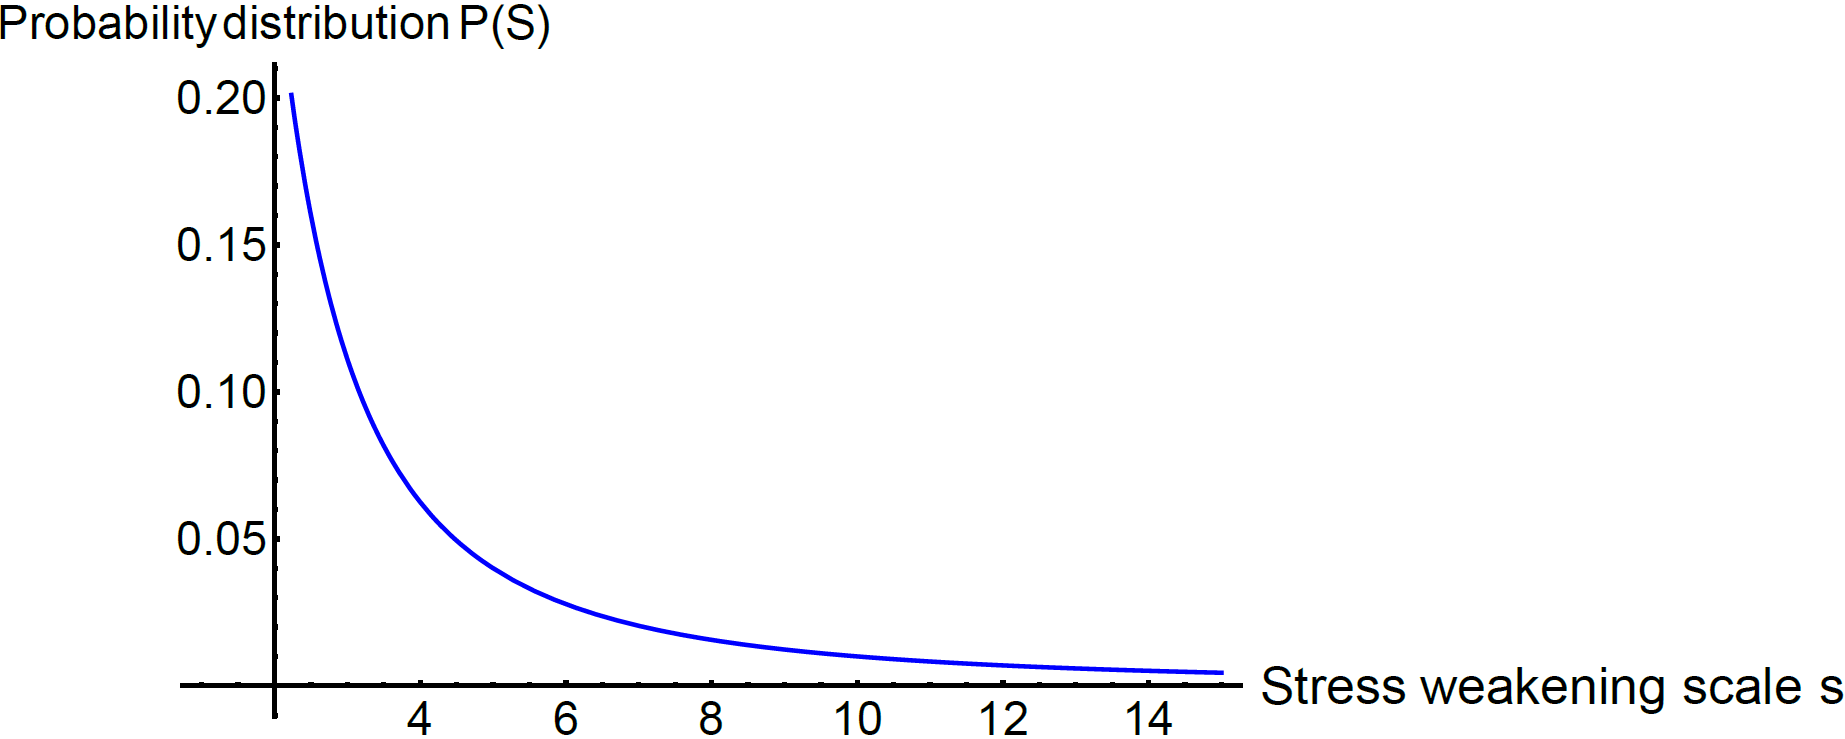
\includegraphics[width=\textwidth]{figures//ps.png} 
		\caption{Weakening scales $s$ probability distribution curve}
		\label{ps}
	\end{figure}
\end{frame}	

\subsection{Yield function with mean stress effect}

\begin{frame}
	\frametitle{Mean stress effect}	
The idea is to consider as in the work of Maitournam and Krebs that the yield limit $\sigma_y$ can be reduced in presence of positive mean stress. The mesoscopic yield function can therefore be written as:
\begin{equation}
f\left(s\right)=||\uline{\uline{S}}(s)-\uline{\uline{b}}(s)||+\left( \lambda \Sigma_H-\sigma_y\right) /s\leqslant 0
\label{yieldfun}
\end{equation}
with $\uline{\uline{S}}(s)$ denoting the deviatoric part of the stress tensor at microscale, and $\uline{\uline{b}}(s)$ the corresponding backstress at the same scale.
\end{frame}	

\subsection{Local plastic model}
\begin{frame}
	\frametitle{Description of the mesoscopic stress state}	

\begin{itemize}
	\item $\dot{\uline{\uline{S}}}(s,M,t)=dev\dot{\uline{\uline{\Sigma}}}(M,t)-\dfrac{E}{1+\nu}\dot{\uline{\uline{\varepsilon}}}^p(s,M,t),$ Taylor-Lin scale transition model.

	\vspace{6pt}	
	\item
	$\dot{\uline{\uline{b}}}(s,M,t)=\dfrac{kE}{E-k} \dot{\uline{\uline{\varepsilon}}}^p(s,M,t),$  kinematic hardening model.

	\vspace{6pt}	
		\item
		$\dot{\uline{\uline{\varepsilon}}}^p(s,M,t)=\gamma\dfrac{\partial f(s,M,t)}{\partial \uline{\uline{S}}}, $ the associated plastic flow rule assuming $\gamma=0$ when $f<0$(elastic) and  $\gamma\geqslant0$ when $f=0$(plastic).
\end{itemize}

	\vspace{6pt}
The local dissipated energy rate per volume at weakening scales $s$  is given by the local entropy dissipation:
$$\dot{w}(s,M,t)=(\uline{\uline{S}}-\uline{\uline{b}})(s,M,t):\uline{\uline{\dot{\varepsilon}}}^p(s,M,t).$$
\end{frame}

\section{Construction of an energy based fatigue approach}
\begin{frame}
	\frametitle{Uniaxial cyclic load}	
	\begin{figure}[h!]
		\centering
		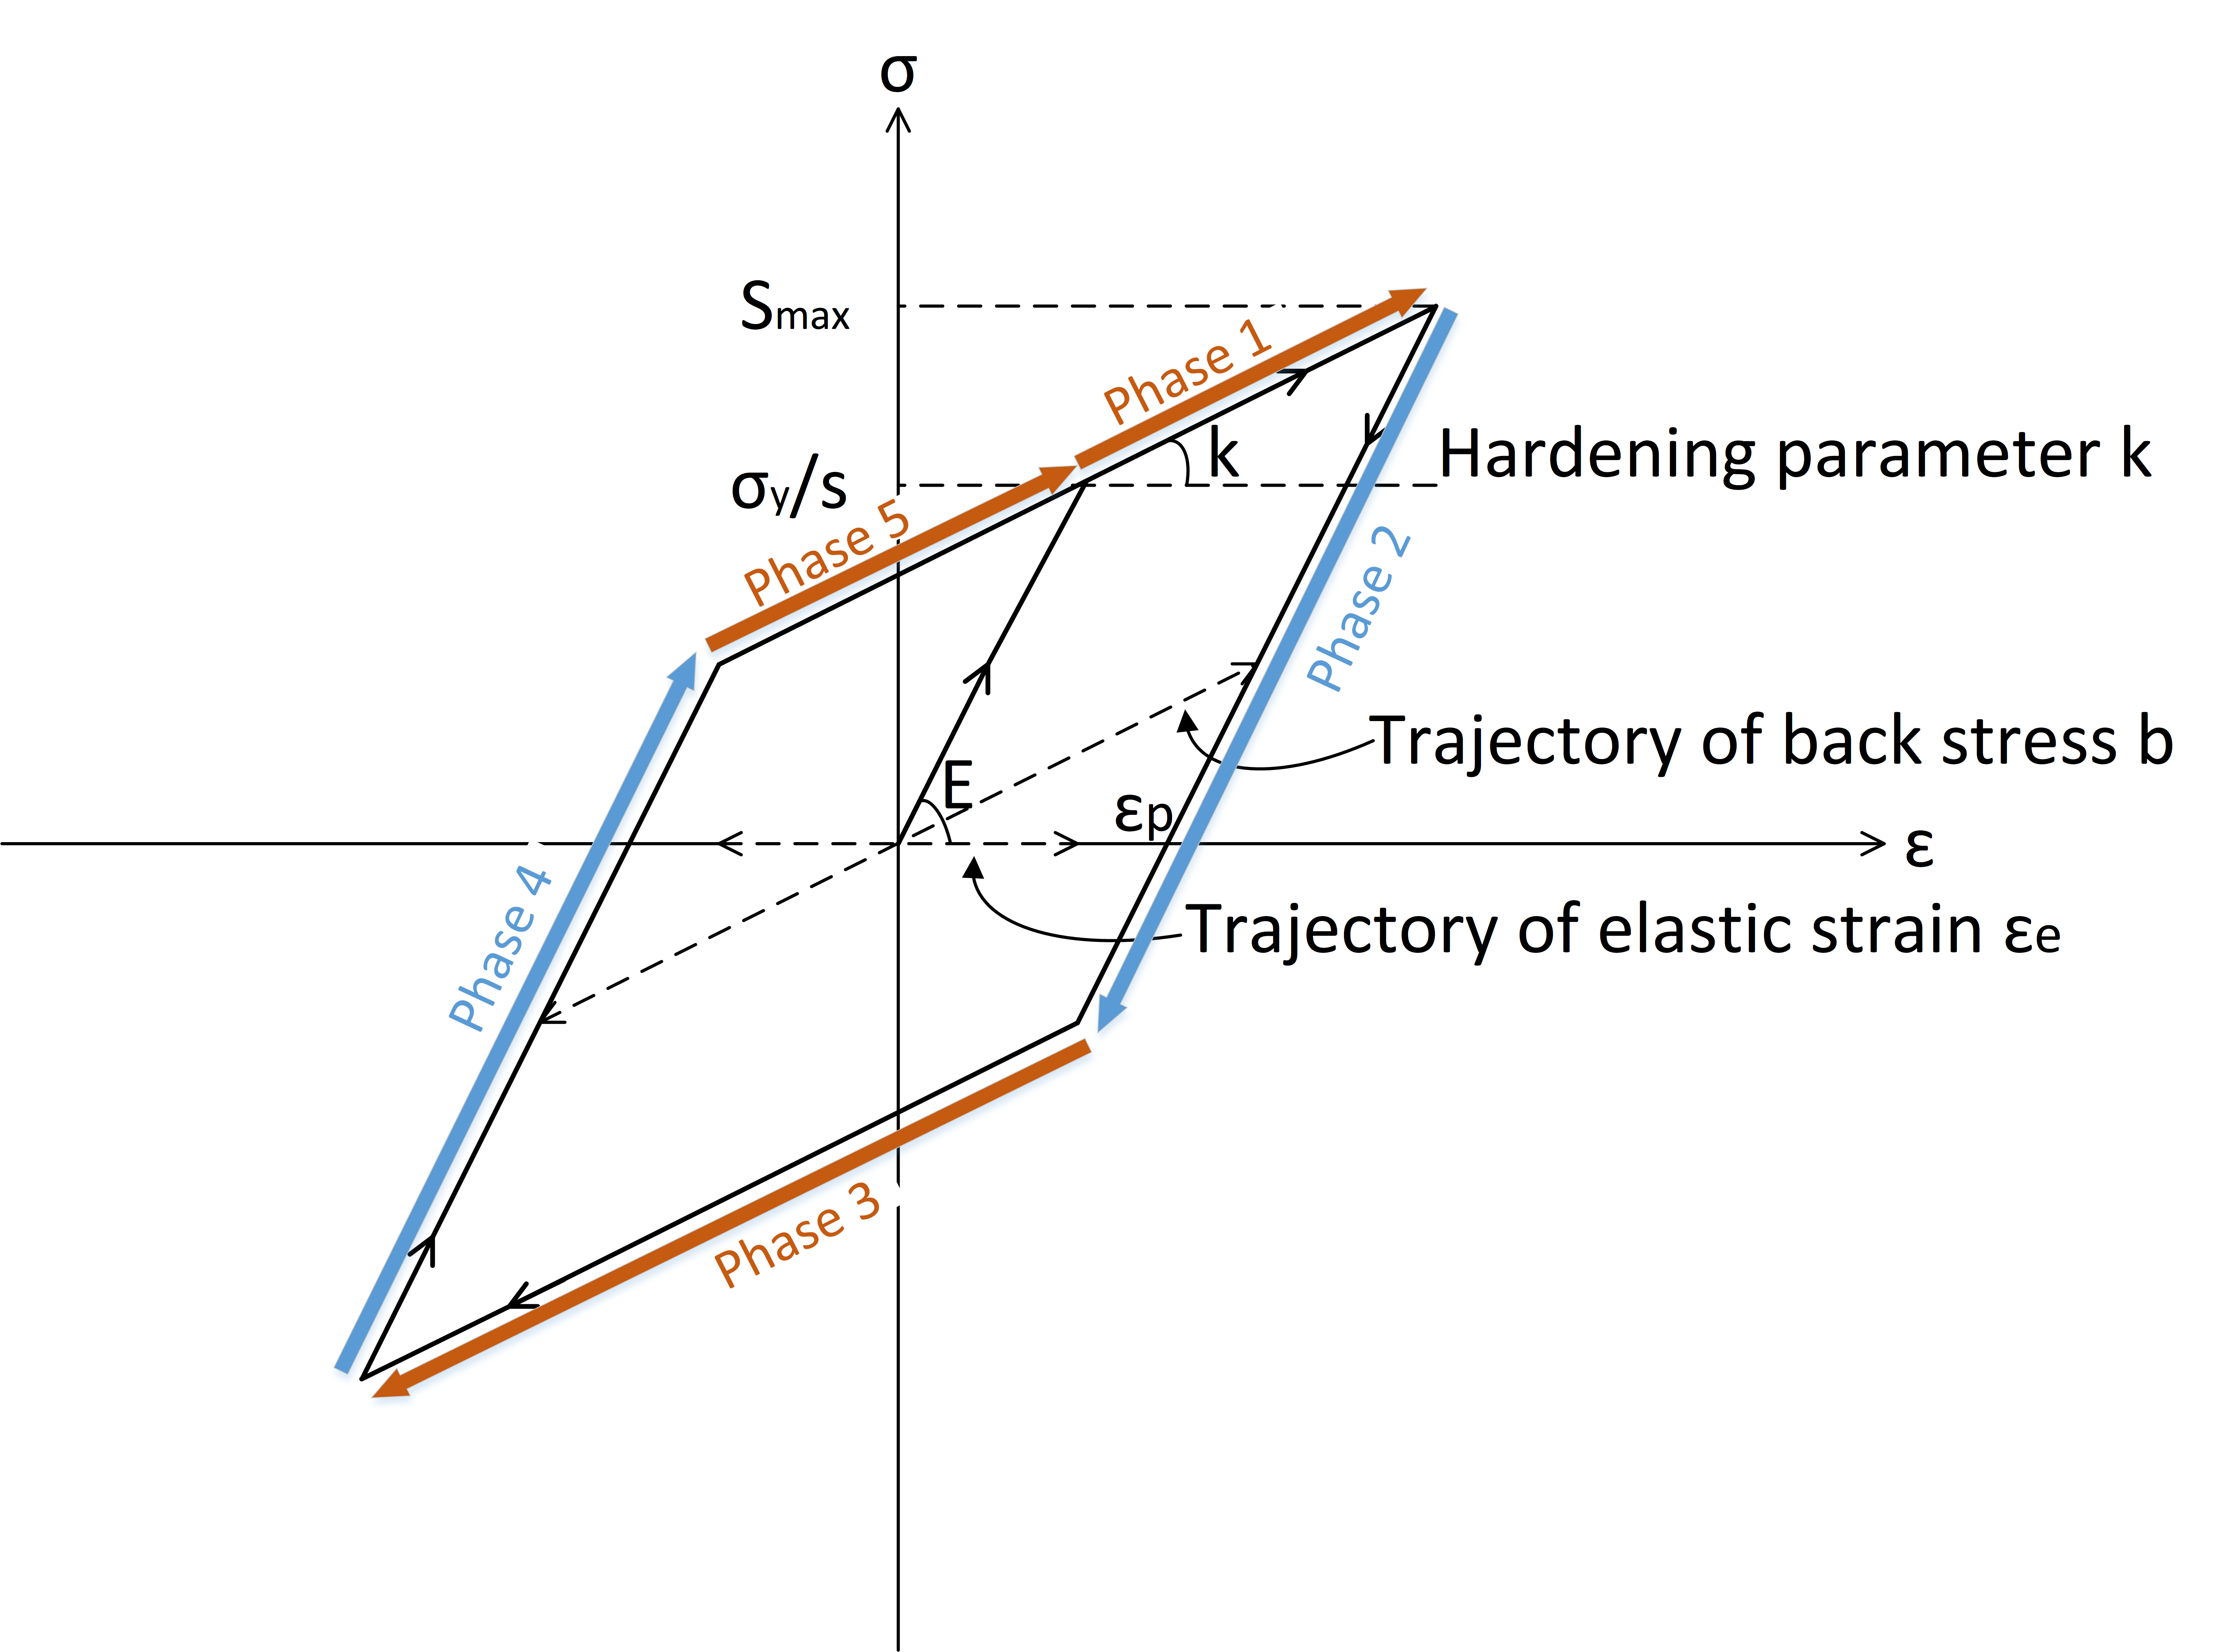
\includegraphics[width=0.9\textwidth]{figures//backstress.png} 
		\label{backstress}
	\end{figure}
\end{frame}	

\begin{comment}
\begin{frame}
	\frametitle{Description of the mesoscopic stress state}	
In uniaxial cyclic loading, there will be 3 kinds of loading patterns:
\begin{enumerate}
	
	\item	Elastic regime, in phase 2 and 4,where $\dot{\uline{\uline{\varepsilon}}}^p(s,M,t)=0$ ,  and $|\uline{\uline{S}}-\uline{\uline{b}}|<\left( \sigma_y-\lambda \Sigma_H\right)/s. $ 
	\vspace{6pt}
	
	\item Plastic regime according to plastic flow rule, with increasing plastic deformation, in phase 5 and 1, where	$\dot{\uline{\uline{\varepsilon}}}^p(s,M,t)=\gamma\dfrac{\uline{\uline{S}}(s)-\uline{\uline{b}}(s)}{||\uline{\uline{S}}(s)-\uline{\uline{b}}(s)||}> 0$ with  $\gamma=\left( dev\dot{\Sigma}\right)\left(\dfrac{kE}{E-k}+\dfrac{E}{1+\nu} \right) ^{-1}$ ,  with $\uline{\uline{S}}-\uline{\uline{b}}=\left( \sigma_y-\lambda \Sigma_H\right)/s$ and $\dot{\uline{\uline{S}}}-\dot{\uline{\uline{b}}}=0.$ 
	\vspace{6pt}
	
	\item Plastic regime in the other direction, in phase 3, there is	$\dot{\uline{\uline{\varepsilon}}}^p(s,M,t)<0$,  then $\uline{\uline{S}}-\uline{\uline{b}}=-\left( \sigma_y-\lambda \Sigma_H\right)/s$ and $\dot{\uline{\uline{S}}}-\dot{\uline{\uline{b}}}=0$ 
	
\end{enumerate}	

\end{frame}	
\end{comment}



\begin{frame}
	\frametitle{Cyclic load calculation}	
	\begin{block}{Energy dissipation at one scale s}
		\begin{itemize}
			\item $dW=(S-b)d\varepsilon^p=\dfrac{(E-k)(1+\nu) }{E(E+k\nu)}\dfrac{\sigma_y-\lambda \Sigma_H}{s}\left(S_{max}-\dfrac{\sigma_y-\lambda \Sigma_H}{s}\right)
			$ (phase 1)
			
			\vspace{6pt}
			\item $dW(phase 1)=dW(phase 5)=\dfrac{1}{2}dW(phase 3).$
	    \end{itemize}	
	\end{block}
	\begin{block}{Total dissipated energy $W$  at all scales during one cycle}
		\begin{equation}
		\begin{split}
		W_{cyc}&=4\int_{\left( \sigma_y-\lambda \Sigma_H\right) /S_{max}}^{\infty}dW(s,M,t)P(s)ds
		\\&=\dfrac{4(E-k)(1+\nu)\left( \beta-1\right) }{ E(E+k\nu)\beta\left( \beta+1\right) }\dfrac{S_{max}^{\beta+1}}{\left( \sigma_y-\lambda \Sigma_H\right) ^{\beta-1}}.
		\end{split}
		\end{equation}
	\end{block}
	
	Where $k$ is the hardening modulus.
\end{frame}	


\section{Damage accumulation}
\begin{frame}
	\frametitle{Generalized damage accumulation}	
	We combine a damage incremental law with relative increment of dissipated energy per unit time:
	\begin{block}{Damage incremental law}	
\begin{equation}
	\delta [1-(1-D)^{\gamma+1}]^{1-\alpha}=\dfrac{\dot{W}}{W_F}\delta t.
	\label{dt}
\end{equation}
	\end{block}
	$W_F$ is the energy threshold of the material.	
		\begin{block}{ Generalized damage accumulation}	
\begin{equation}\dot{W}(M,t)=\int_{s=1}^{\infty}\dot{w}(s,M,t)P(s)ds=\int_{s=1}^{\infty}\left(\uline{\uline{S}}-\uline{\uline{b}} \right) (s,M,t):\uline{\uline{\dot{\varepsilon}^p}}(s,M,t)P(s)ds.
\end{equation}
		\end{block}
\end{frame}	

\section{Loop on time and scales}
\subsection{Integration rules for $\dot{W}$ and $\delta D$}

\begin{frame}
\frametitle{Integration rules}
	\begin{block}{}	
\begin{itemize}
\item There are certain limitations of cycle counting method. Firstly we need a load history decomposition in cycles. Secondly in real life the perfect close loop cycle is hardly applicable.
					
\vspace{6pt}
\item We propose in a more general method which can be integrated using a step by step strategy. 
					
\vspace{6pt}
\item Instead of doing the scale integration directly which can be difficult for complex loading, the Gaussian Quadrature rule with Legendre points is used to give the value of local dissipated energy rate.
\end{itemize}	
\end{block}
\end{frame}	

\begin{frame}
	\frametitle{Integration rules}
The dissipated energy summed on all scales is:
\begin{equation}
	\begin{split}
		\dot{W}&=\int_{1}^{\infty}\dot{w}(s) (\beta-1)(s)^{-\beta}ds
			\\&=\frac{1}{2}\int_{-1}^{1}\dot{w}\left[  \left( \frac{x+1}{2}\right) ^{\frac{1}{1-\beta}}\right] dx
			\\&\approx\frac{1}{2}\sum_{i}\omega_id\dot{w}\left[  \left( \frac{x_i+1}{2}\right) ^{\frac{1}{1-\beta}}\right],
	\end{split}
	\label{allscale}
\end{equation}

\vspace{6pt}
where $\omega_i$ and $x_i$ are respectively the weights and nodes of the Gauss Legerndre integration rule used for the numerical integration. In this work, we used 25 points.
\end{frame}

\subsection{Regime determination under multiple scales}
\begin{frame}
	\frametitle{Regime determination}
	The material could be both in elastic and plastic regime under different scales.
	\begin{block}{Elastic regime:}	
\noindent
There we have
$\dot{\uline{\uline{\varepsilon}}}^p=0$, $\dot{\uline{\uline{b}}}=0$ and $\dot{\uline{\uline{S}}}=dev\dot{\uline{\uline{\Sigma}}}$, so
$$\dot{\uline{\uline{S}}}-\dot{\uline{\uline{b}}}=dev\dot{\uline{\uline{\Sigma}}},$$ 
yielding
\begin{equation}
\left( \uline{\uline{S}}-\uline{\uline{b}}\right) (t+dt)=\left( \uline{\uline{S}}-\uline{\uline{b}}\right) (t)+dev\dot{\uline{\uline{\Sigma}}}dt:=\left(  \uline{\uline{S}}-\uline{\uline{b}}\right)_{trial}(s,t+dt).
\label{trial}
\end{equation}
We are in elastic regime at scale $s$ as long as we satisfy
$$\left( \uline{\uline{S}}-\uline{\uline{b}}\right) (t+dt)\leqslant\left( \sigma_y-\lambda \Sigma_H\right)/s.$$	
	\end{block}
\end{frame}	

\begin{frame}
	\frametitle{Regime determination}
	\begin{block}{Plastic regime:}	
\begin{numcases}{}
\dot{\uline{\uline{\varepsilon}}}^p=\gamma\dfrac{\uline{\uline{S}}-\uline{\uline{b}}}{\left| \left|\uline{\uline{S}}-\uline{\uline{b}}\right| \right|}, \gamma>0, & plastic   flow,\\
\left| \left|\uline{\uline{S}}-\uline{\uline{b}}\right| \right|=\left( \sigma_y-\lambda \Sigma_H\right)/s, & yield   limit,\\
\left( \uline{\uline{S}}-\uline{\uline{b}}\right) :\left( \dot{\uline{\uline{S}}}-\dot{\uline{\uline{b}}}\right) =0, & yield   limit   time invariance,\\
\dot{\uline{\uline{b}}}=\dfrac{kE}{E-k}\dot{\uline{\uline{\varepsilon}}}^p, & kinematic   hardening  rule,\\
\dot{\uline{\uline{S}}}=dev\dot{\uline{\uline{\Sigma}}}-\dfrac{E}{1+\nu} \dot{\uline{\uline{\varepsilon}}}^p, & localisation  rule.
\end{numcases}
	\end{block}
\end{frame}	


\begin{frame}
	\frametitle{Regime determination}
	
	\begin{block}{In all cases, we get in plastic regime:}	
\begin{equation}
\left( \uline{\uline{S}}-\uline{\uline{b}}\right) (s,t+dt)=\dfrac{\left( \uline{\uline{S}}-\uline{\uline{b}}\right)_{trial} (s,t+dt)}{1+\eta},
\end{equation}

$$\eta=max\left\lbrace \underbrace{0}_{elastic\; regime}, \underbrace{\dfrac{\left| \left|\uline{\uline{S}}-\uline{\uline{b}}\right| \right|_{trial}}{\left( \sigma_y-\lambda \Sigma_H\right)/s}-1}_{plastic \; regime\; when\; this\; number\; is\; positive}\right\rbrace. $$
	\end{block}
 That is to say, when the structure is in elastic regime at time $t$ and scale $s$, we have $\left( \uline{\uline{S}}-\uline{\uline{b}}\right)(s,t)=\left( \uline{\uline{S}}-\uline{\uline{b}}\right)_{trial} (s,t)$. Otherwise, if  the norm of $\left( \uline{\uline{S}}-\uline{\uline{b}}\right)_{trial} (s,t)$ is greater than the local yield limit $\left( \sigma_y-\lambda \Sigma_H\right)/s$, $\left( \uline{\uline{S}}-\uline{\uline{b}}\right)(s,t)$ will be projected on the yield limit. 	
\end{frame}	

\begin{frame}
	\frametitle{Regime determination}
	\begin{block}{Final expression of energy dissipation during time step dt }	
	\begin{equation}
	\begin{split}
	W&=\dot{W}dt
	\\&=\frac{1}{2}\sum_{i}\omega_i\dot{w}\left[  \left( \frac{x+1}{2}\right) ^{\frac{1}{1-\beta}}\right]dt
	\\&=\dfrac{(E-k)(1+\nu) }{2E(E+k\nu)}\sum_{i}\omega_i\left\langle  \left| \left|\uline{\uline{S}}-\uline{\uline{b}}\right| \right|_{trial}-\dfrac{\sigma_y-\lambda \Sigma_H}{\left( \dfrac{x_i+1}{2}\right) ^{\frac{1}{1-\beta}}}\right\rangle \dfrac{\sigma_y-\lambda \Sigma_H}{\left( \dfrac{x_i+1}{2}\right) ^{\frac{1}{1-\beta}}}.
	\end{split}
	\label{finaldw}
	\end{equation}
	\end{block}

$$g_{n+1}=g_n+\dfrac{\dot{W}dt}{W_F}=g_n+\dfrac{W}{W_F},$$

with $D_n=\left[1-\left(1-g_n^{\frac{1}{1-\alpha}} \right)^{\frac{1}{\gamma+1}}  \right] $.

\end{frame}	

\section{Application}
\subsection{One dimensional application to simple cyclic data}

\begin{frame}
	\frametitle{Material parameters}
	The test is performed on a sinusoidal axial load $\Sigma=Csin(t)$, giving the deviatoric amplitude $S_{max}=\sqrt{\dfrac{2}{3}}C$.
\begin{table}[!h]
	\centering
	\begin{tabular}{ll}
		\hline
		\textbf{Parameters}                                         & \textbf{Value}                    \\ \hline
		Load                                                              & $\Sigma=5e8sin(t)$ Pa                  \\
		Young's modulus                                             & $E=2e11$ Pa                       \\
		Hardening parameter                                         &  $k=6e8$ Pa \\
		Weakening scales distribution exponent                      & $\beta=3$                             \\
		Hydrostatic pressure sensitivity                            & $\lambda=0.5$                     \\
		Macroscopic yield stress                                    & $\sigma_y=6.38e8$ Pa              \\
		Mean stress                                        & $\Sigma_H=0$ Pa                     \\
		Material parameter from Chaboche law(Wohler curve exponent) & $\gamma=0.5$                        \\
		Non-linearity of damage accumulation & $\alpha=0.8$                        \\
		Initial damage                                              & $D=0$                          \\
		Initial time                                                & $t=0$ s                            \\
		Dissipated energy to failure per unit volume                & $W_F=3e6$ J                       \\
		Looping step                                           & 1e-4 s              \\ \hline
	\end{tabular}
	\caption{Material parameters in a simple cyclic load }
	\label{Sin}
\end{table}
\end{frame}	


\begin{frame}
	\frametitle{Sinusoidal test}
\begin{figure}[!h]
	\centering
	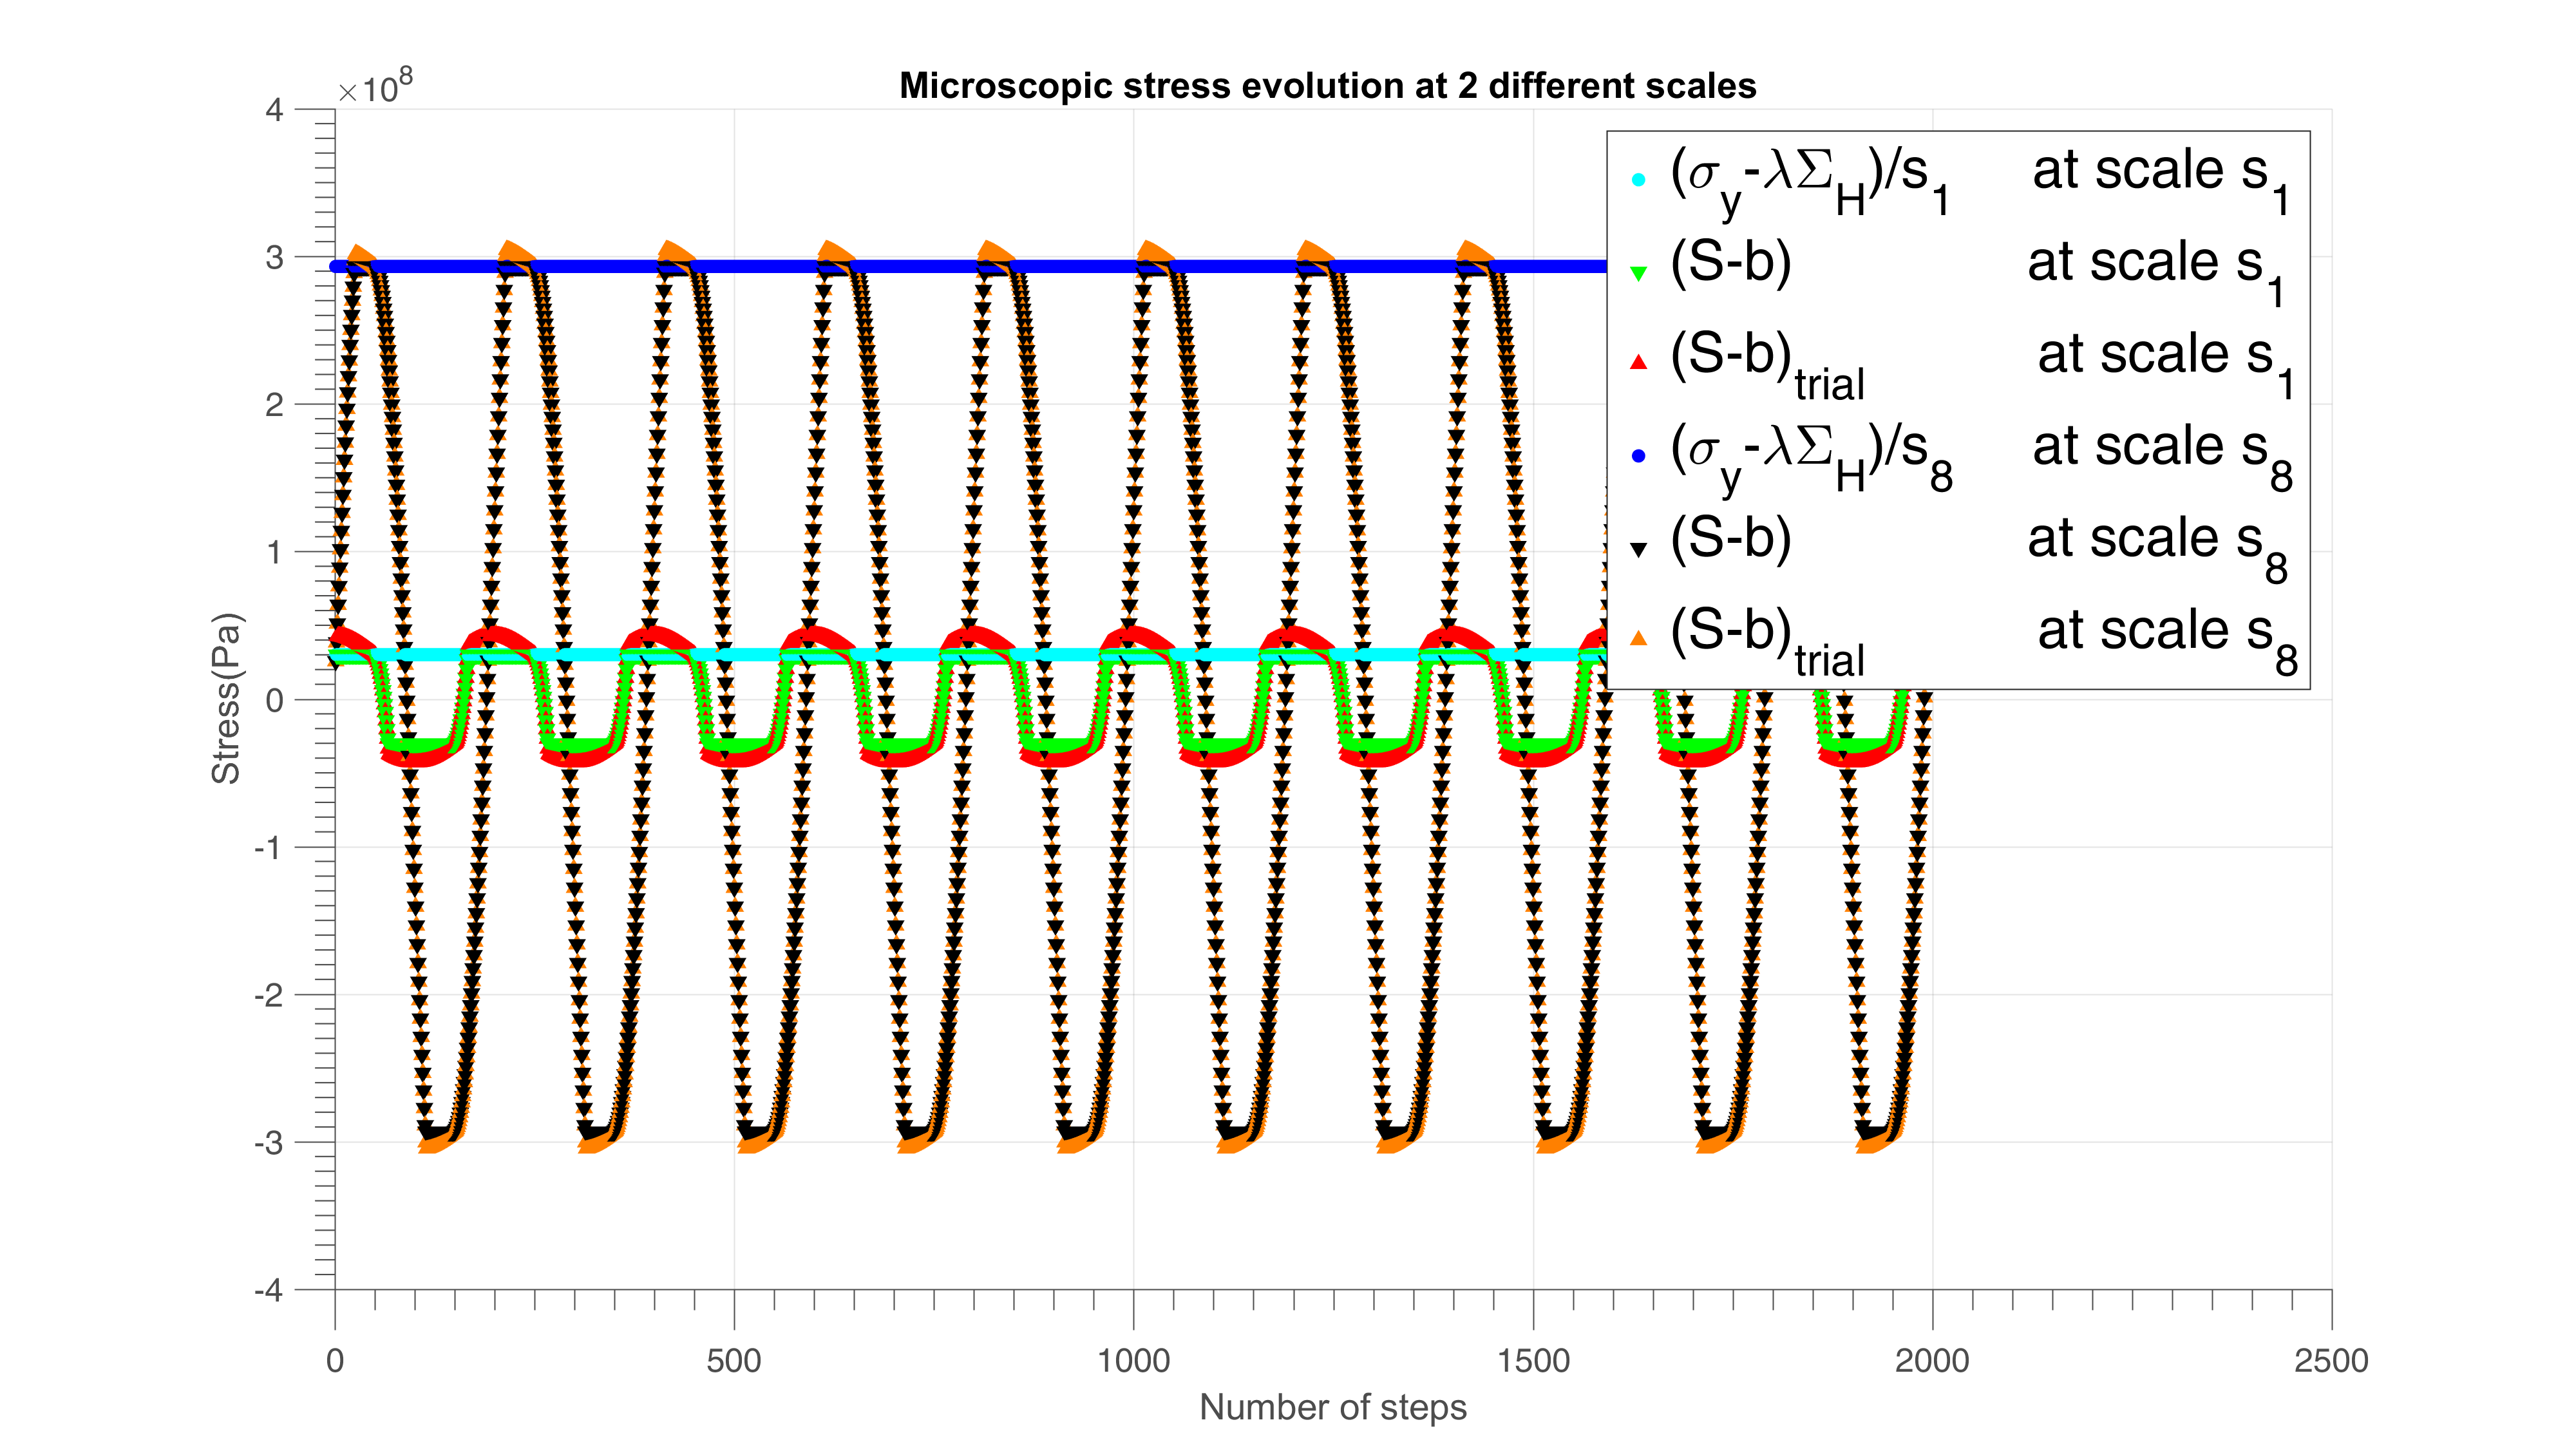
\includegraphics[width=\textwidth]{figures//trialsin.png} 
	\caption{Microscopic $\left( \uline{\uline{S}}-\uline{\uline{b}}\right)_{trial}$ and $\left( \uline{\uline{S}}-\uline{\uline{b}}\right)$ evolution with time under different weakening scales in sinusoidal load($s_1=21.21657929229650$ and $s_8=2.176132808422946$)}
	\label{trialsin}
\end{figure}
\end{frame}	
\begin{frame}
	\frametitle{Sinusoidal test}
\begin{figure}[!h]
	\centering
	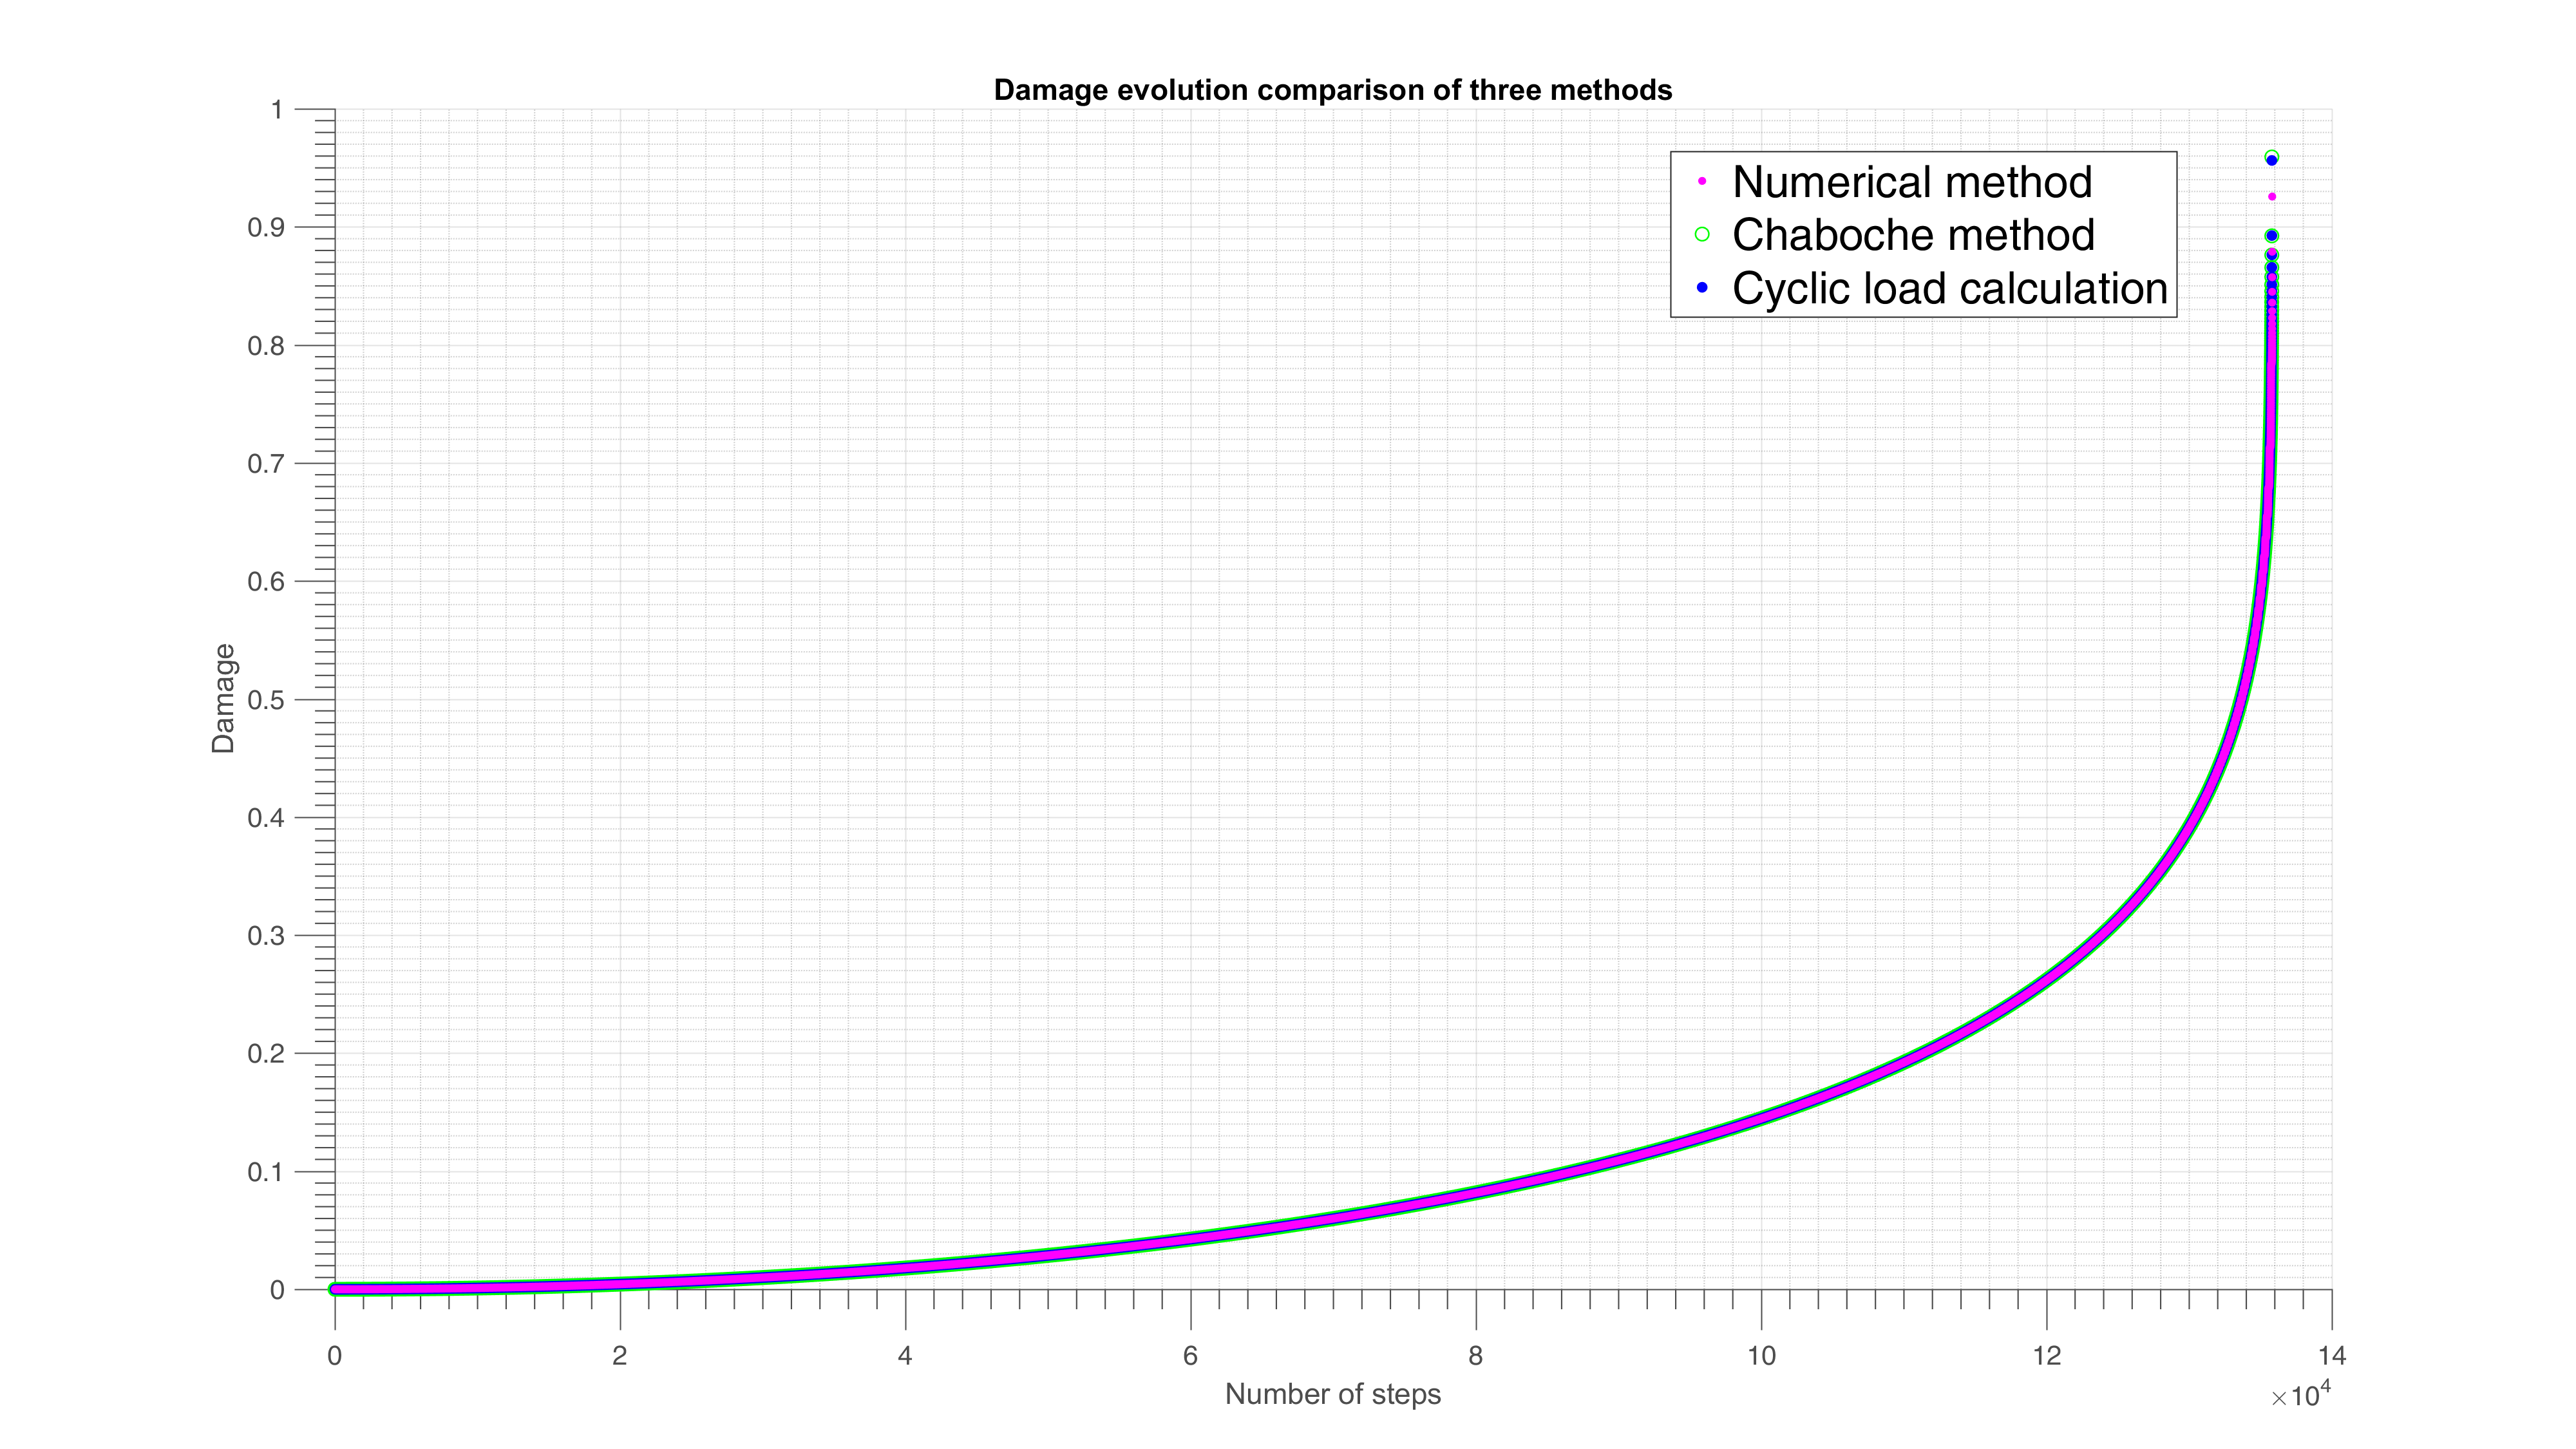
\includegraphics[width=\textwidth]{figures//damagesin.png} 
	\caption{Damage evolution with time under sinusoidal load with two different methods}
	\label{damsin}
\end{figure}
\end{frame}	

\begin{frame}
	\frametitle{Convergence test}
	Because the step by step damage accumulation grows in a power law, so the amplitude of difference grows with time. However, the difference between the two methods swing around 0 so we could consider the numerical method converges in cyclic load calculation method.
	\begin{figure}[htbp]
		\begin{minipage}[t]{0.48\linewidth}
	\centering
	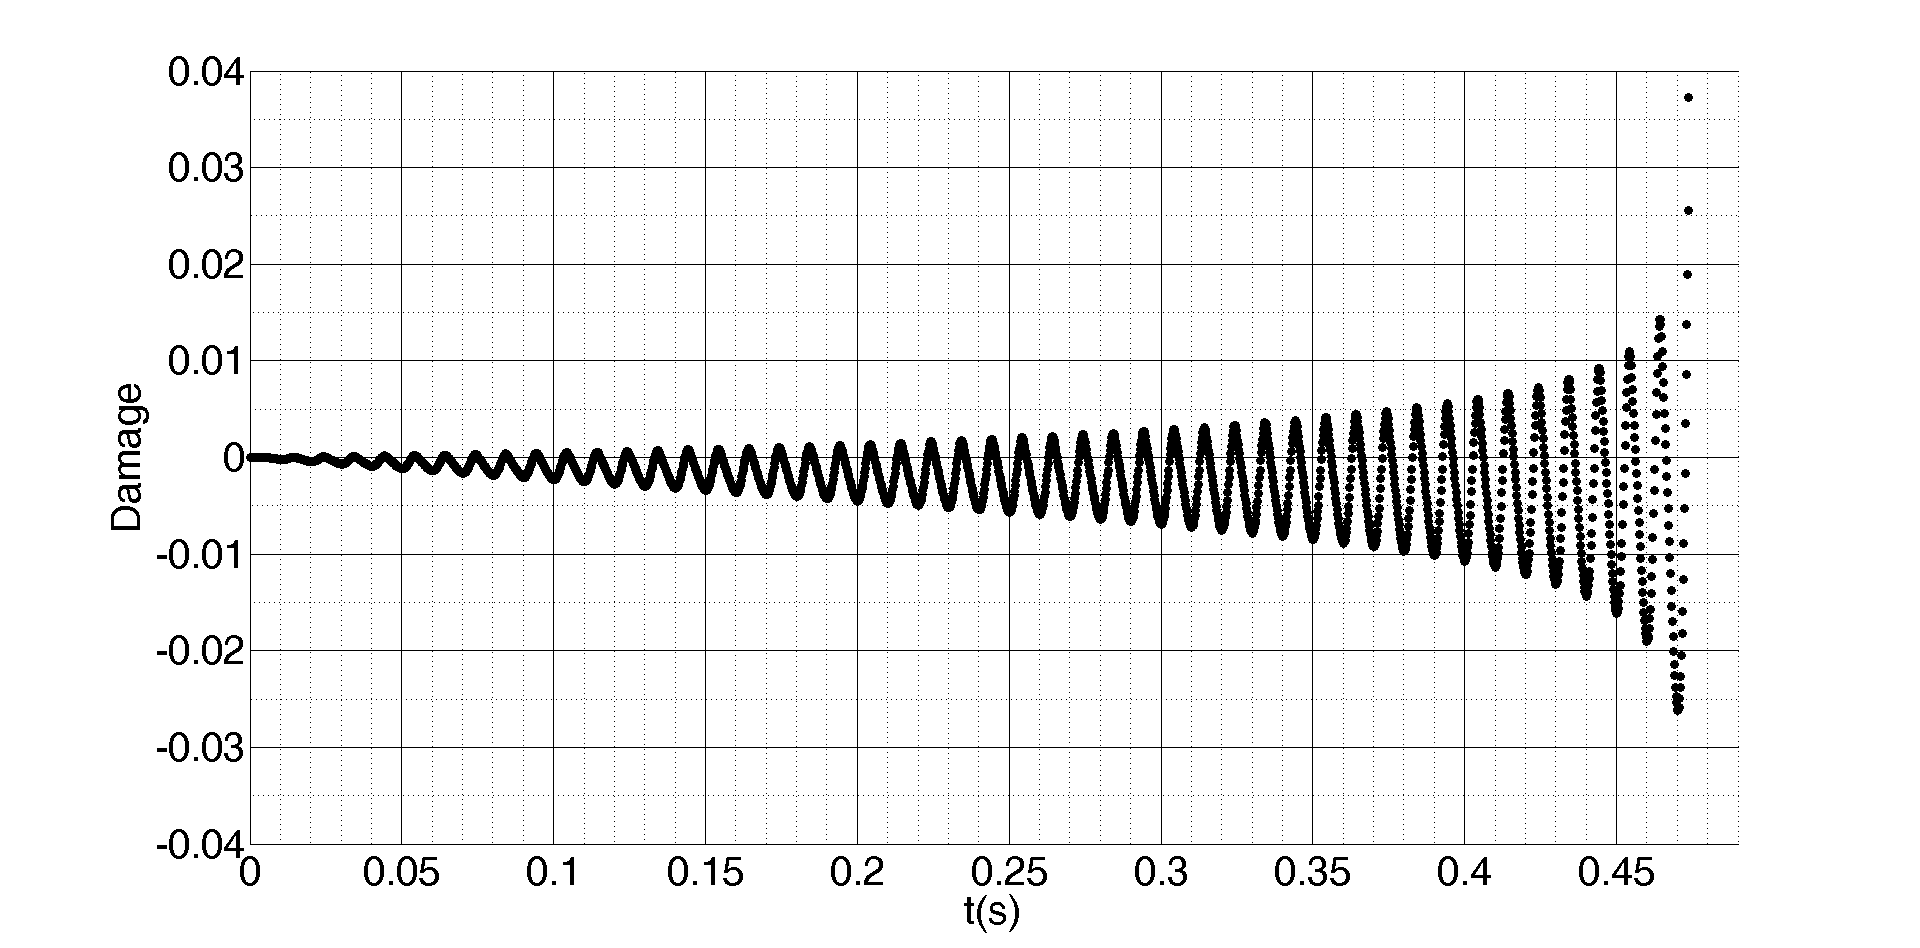
\includegraphics[width=\textwidth]{figures//NCdiff100.png} 
	\caption{Difference between cyclic load calculation and numerical method as function of time(time step=1/5000s)}
	\label{NCdiff100}
		\end{minipage}
		\begin{minipage}[t]{0.48\linewidth}
	\centering
	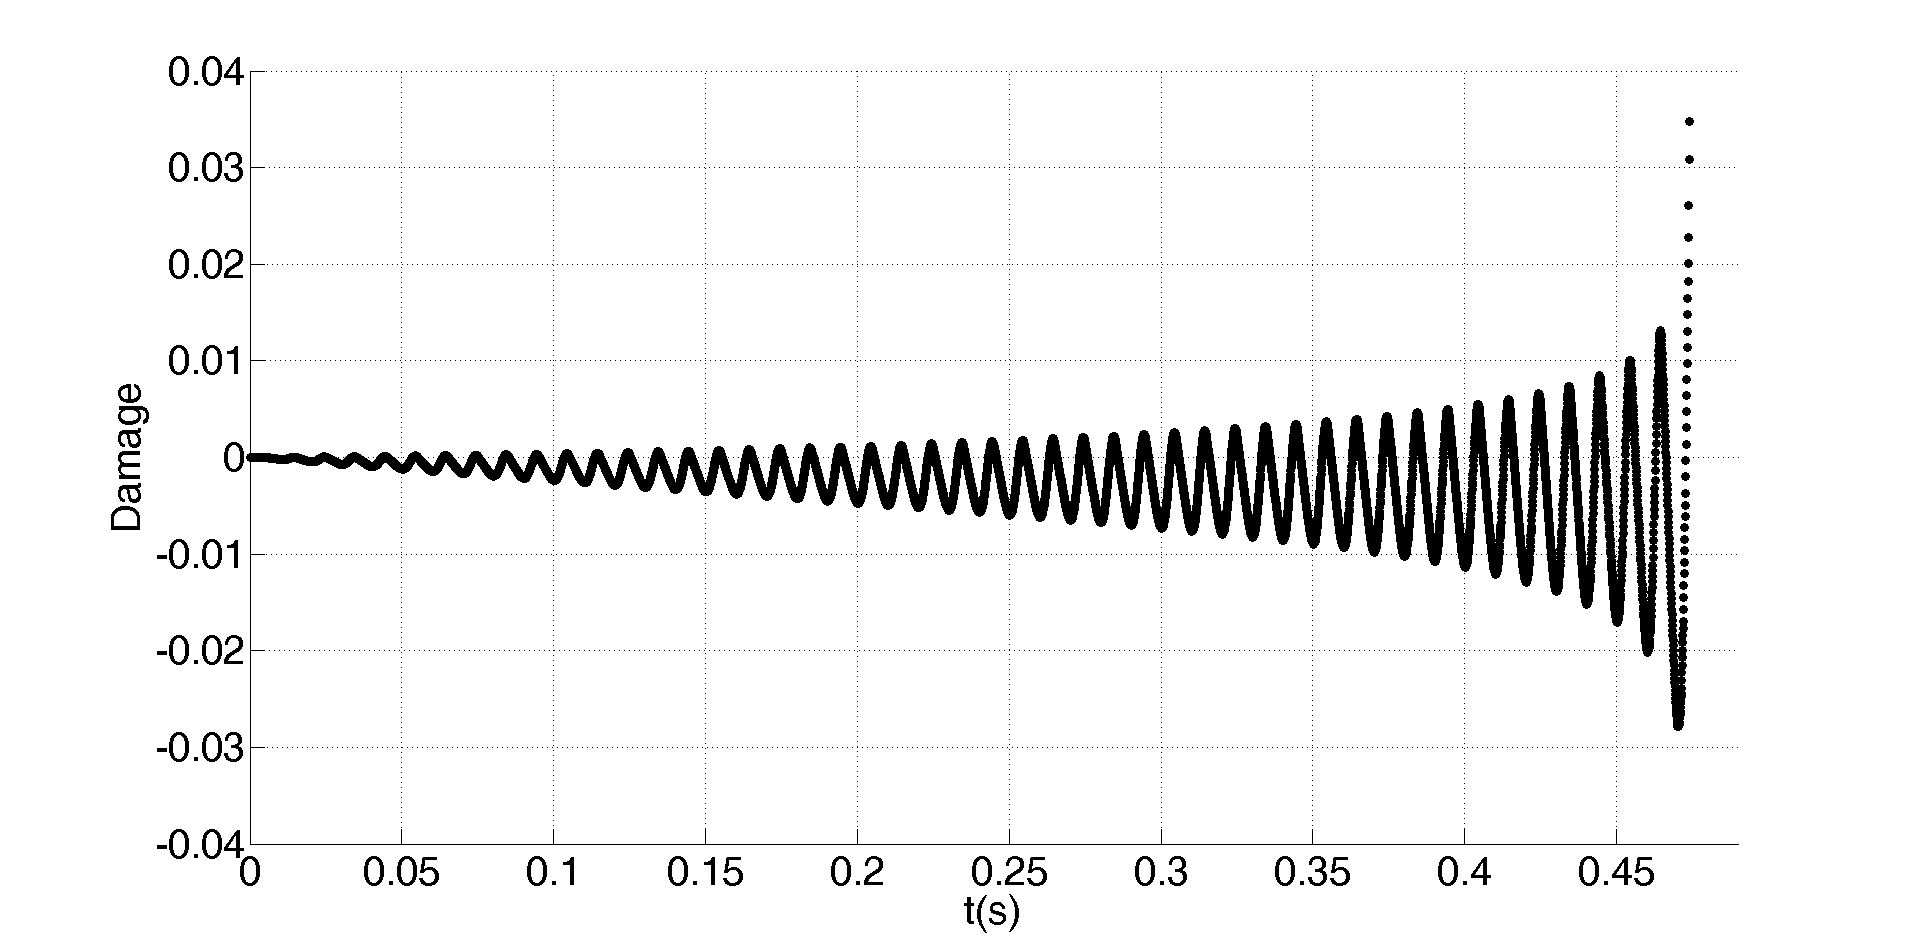
\includegraphics[width=\textwidth]{figures//NCdiff300.png} 
	\caption{Difference between cyclic load calculation and numerical method as function of time(time step=1/15000s)}
	\label{NCdiff300}
		\end{minipage}
	\end{figure} 
\end{frame}	
\subsection{One dimensional application to PSA data}

\begin{frame}
	\frametitle{One dimensional application}
\begin{figure}[!h]
	\centering
	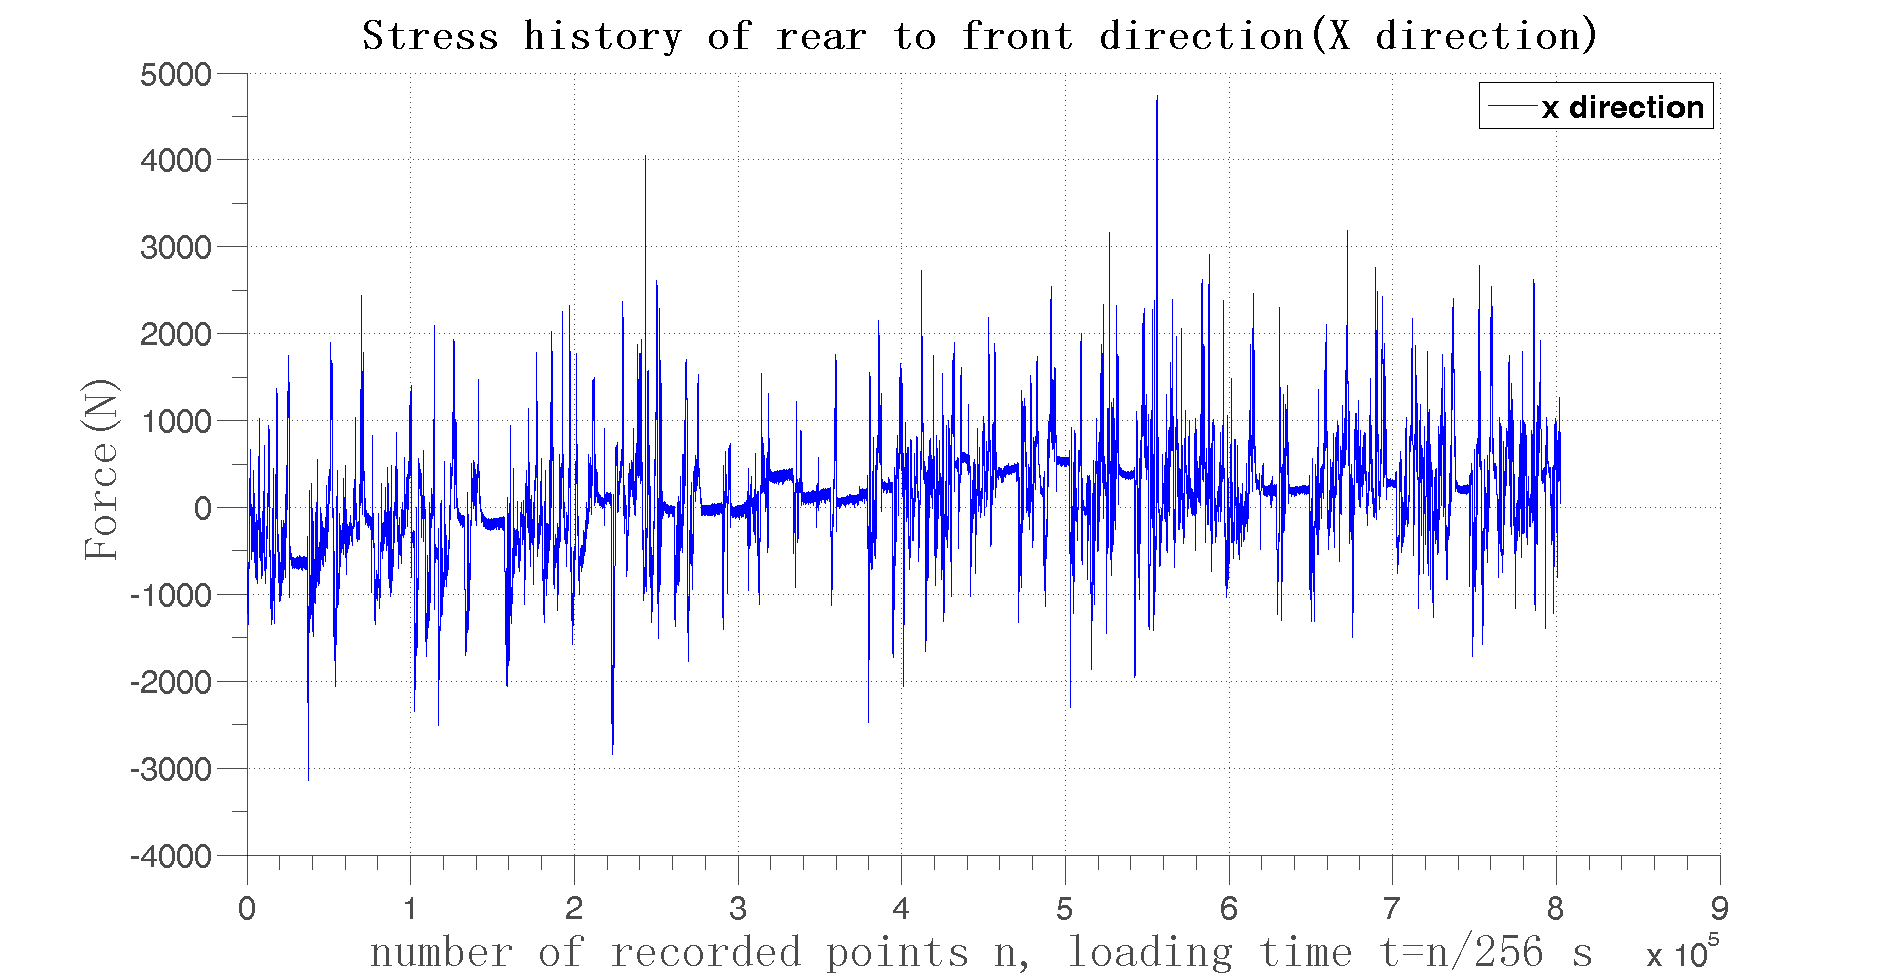
\includegraphics[width=\textwidth]{figures//x.png} 
	\caption{Loading history of X direction, force vs the record index n, with 256 sample recorded per second}
	\label{x}
\end{figure}
\end{frame}	

\begin{frame}
	\frametitle{One dimensional application}
 	\begin{block}{Numerical methods:}

			\begin{itemize}
				\item 	The sample recording rate is 256 per second. In order to accumulate damage using very small steps, we have created 10 additional points between every 2 recorded points by linear interpolation.
				\vspace{6pt}
				\item The force on wheel is firstly considered as under uniaxial loading $F_x$. Here we temporally set $\Sigma_x=F_x/A$ where $A=\dfrac{1}{6e5} m^2$ is the area of force, and $W_F=3e6 J$. 
		\end{itemize}
 
	\end{block}
\end{frame}	



\begin{frame}
	\frametitle{One dimensional application}
\begin{figure}[!h]
	\centering
	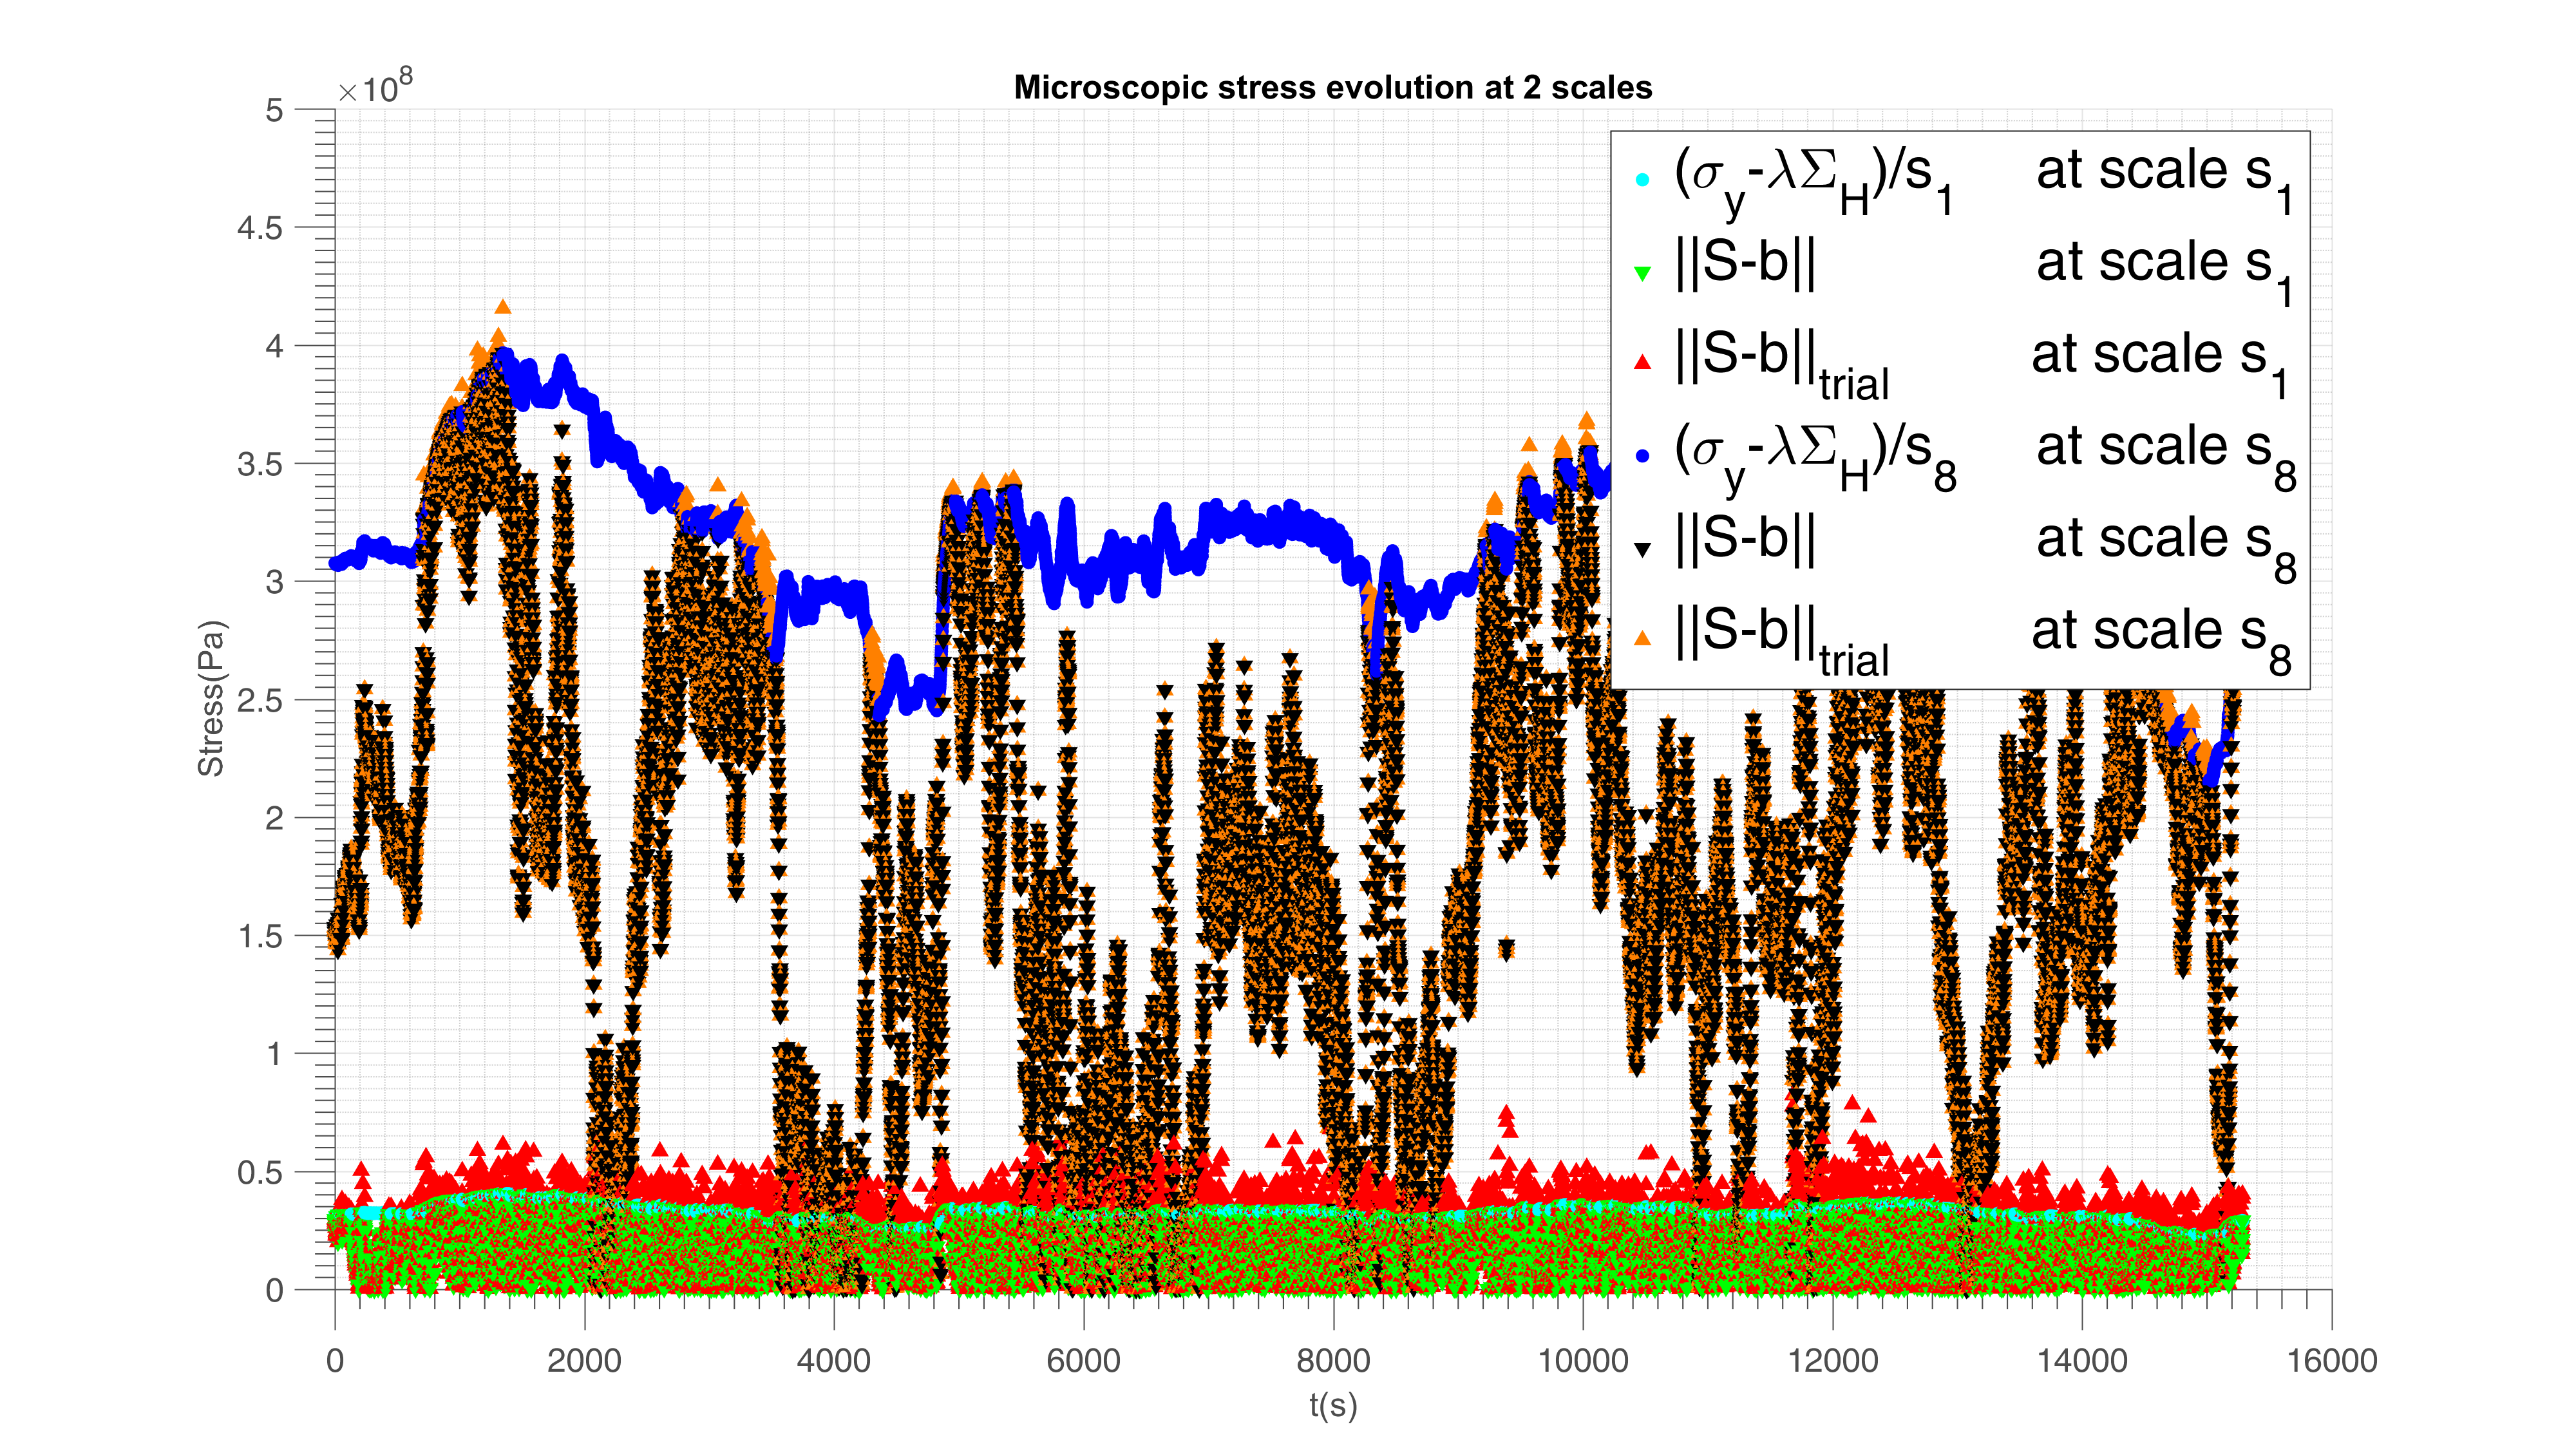
\includegraphics[width=\textwidth]{figures//trialreal1d1.png} 
	\caption{$\left\|  \uline{\uline{S}}-\uline{\uline{b}}\right\| _{trial}$ and $\left\| \uline{\uline{S}}-\uline{\uline{b}}\right\|$ evolution with time under different weakening scales in PSA load history}
	\label{trialreal}
\end{figure}
\end{frame}	

\begin{frame}
	\frametitle{One dimensional application}
	\begin{figure}[!h]
		\centering
		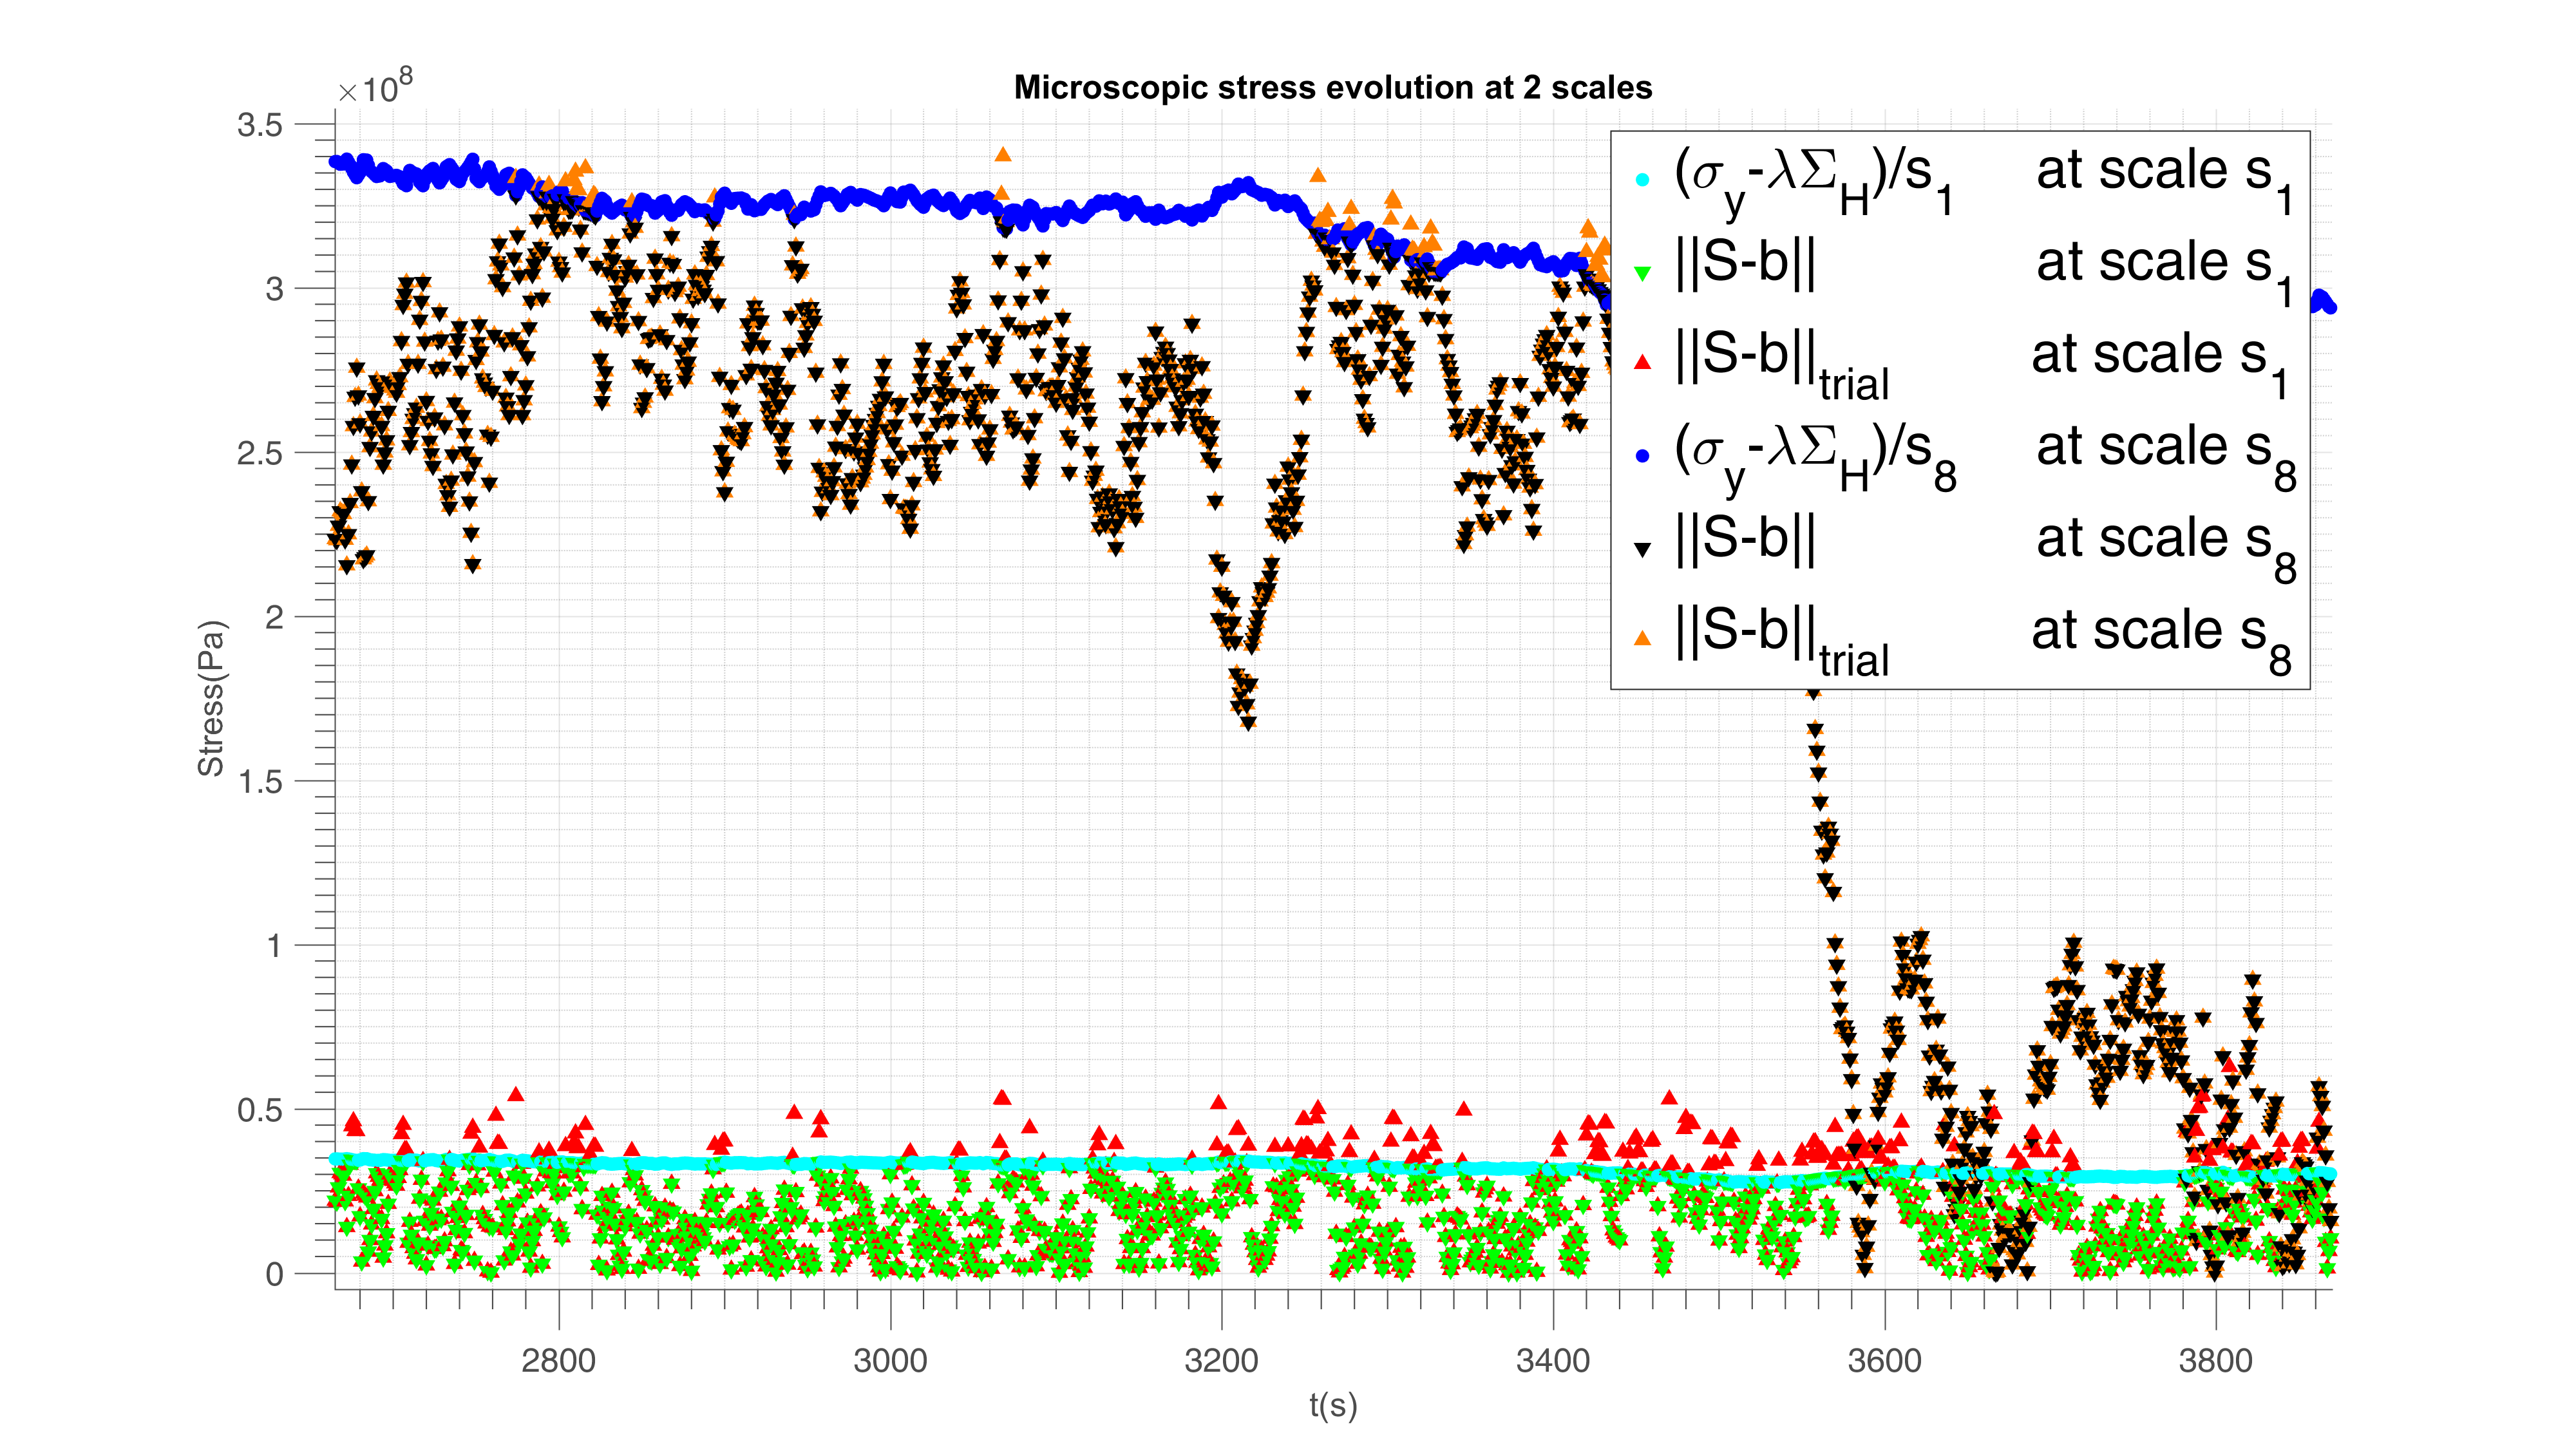
\includegraphics[width=\textwidth]{figures//trialreal1d2.png} 
		\caption{Circled area magnification where there is more $\left\| \uline{\uline{S}}-\uline{\uline{b}}\right\|_{trial}>\sigma_y$(plasticity) at scale $s_1$ than at $s_8$}
		\label{trialreal1d3}
	\end{figure}
\end{frame}	

\begin{frame}
	\frametitle{One dimensional application}
\begin{figure}[!h]
	\centering
	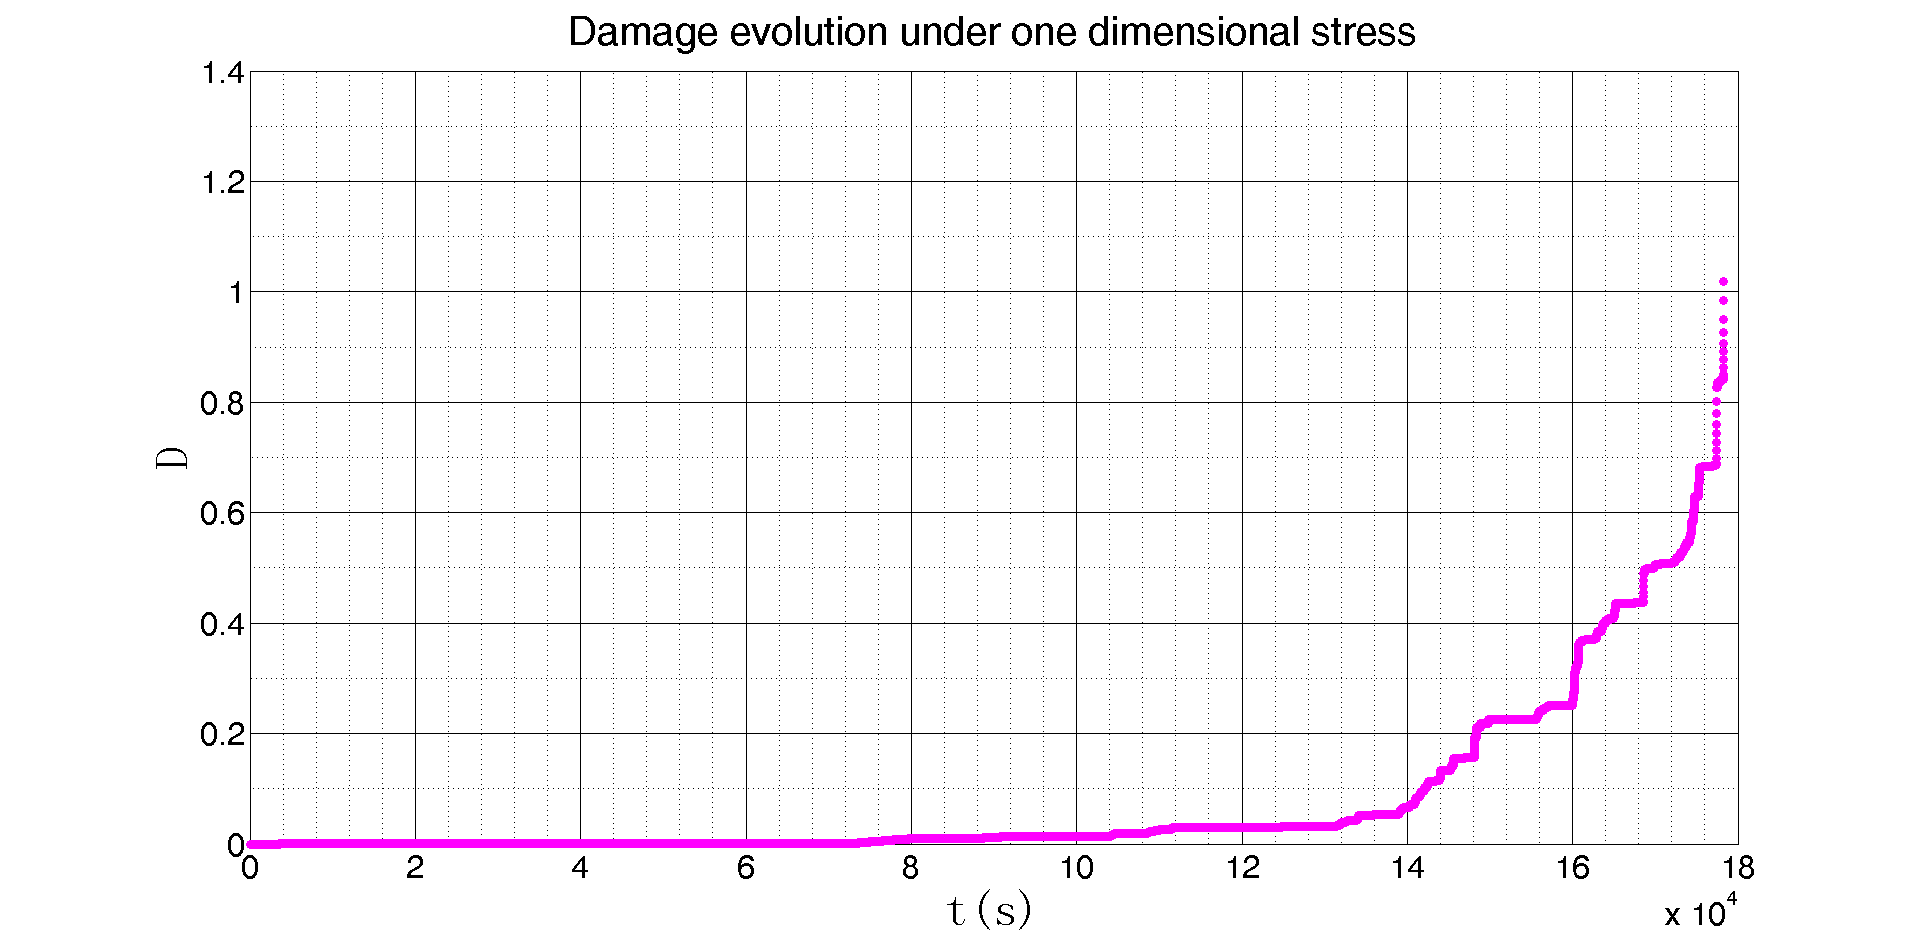
\includegraphics[width=\textwidth]{figures//damage1d.png} 
	\caption{Damage evolution with time at one dimension PSA load history}
	\label{damage1d}
\end{figure}
\end{frame}	



 \subsection{Multi-dimensional application to PSA data}
\begin{frame}
	\frametitle{Multi-dimensional application}
 We now consider a situation where we have force recorded measured in 3 different directions as shown in \figref{xyz}.
 \begin{figure}[!h]
 	\centering
 	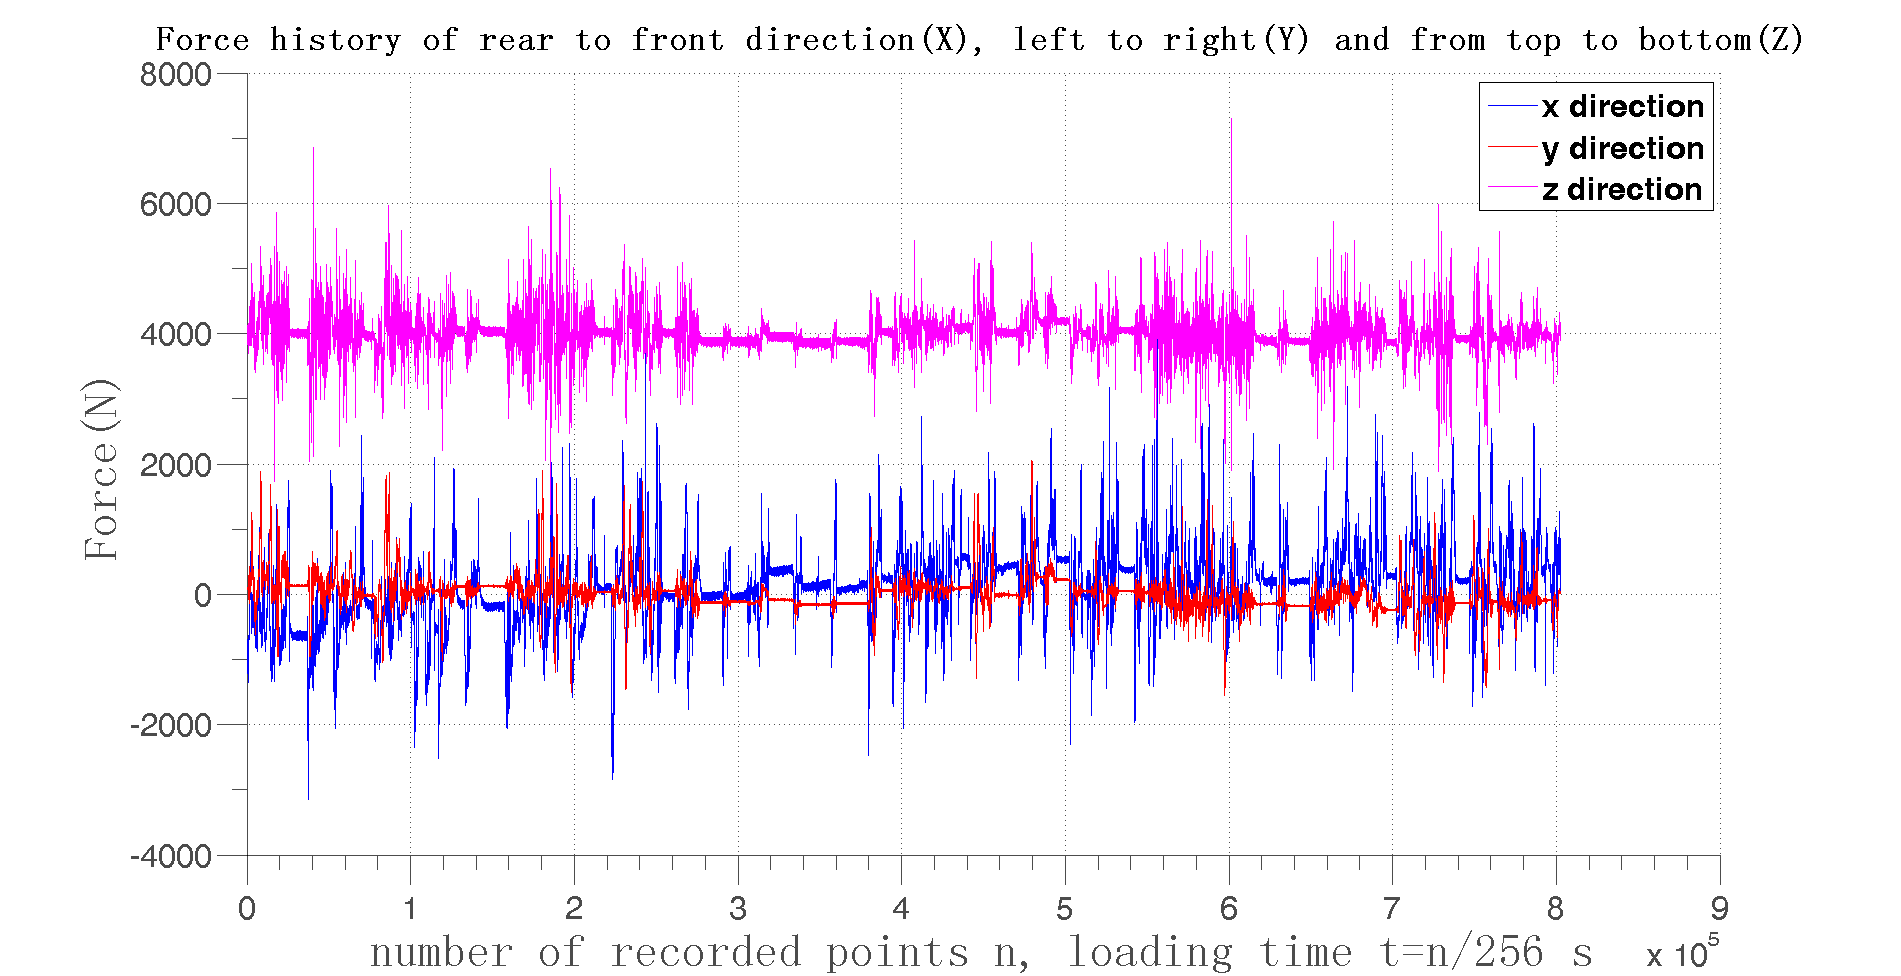
\includegraphics[width=\textwidth]{figures//xyz.png} 
 	\caption{Loading history of 3 different directions}
 	\label{xyz}
 \end{figure}
\end{frame}	

\begin{frame}
	\frametitle{Multi-dimensional application}
 In real case, the vertical force $F_z$ is much larger than the axial and horizontal forces $F_x$ and $F_y$. However, in order to investigate large domains of interest, we first scale the axial and horizontal forces to reach comparable impact and transform them in principal stresses $c_x\dfrac{F_x}{A}$ applied along the stress principle vector $\uline{e}_\alpha$(respectively $\uline{e}_\beta$) that we choose randomly. We therefore consider the following macroscopic stress tensor:
 \begin{equation}
 \uline{\uline{\Sigma}}=\dfrac{F_z(t)}{A}\uline{e}_1\otimes \uline{e}_1+c_x\dfrac{F_x(t)}{A}\uline{e}_{\alpha}\otimes \uline{e}_{\alpha}+c_y\dfrac{F_y(t)}{A}\uline{e}_{\beta}\otimes \uline{e}_{\beta}
 \label{tensor1}
 \end{equation}
 where $\uline{e}_{\alpha}$  and $\uline{e}_{\beta}$ are principal vectors whose spherical coordinate are $\theta_x$, $\varphi_x$,  $\theta_y$ and $\varphi_y$ respectively:
 $$\uline{e}_{\alpha}=cos\theta_x\uline{e}_1+sin\theta_xcos\varphi_x\uline{e}_2+sin\theta_xsin\varphi_x\uline{e}_3,$$
 $$\uline{e}_{\beta}=cos\theta_y\uline{e}_1+sin\theta_ycos\varphi_y\uline{e}_2+sin\theta_ysin\varphi_y\uline{e}_3.$$
 
 \begin{table}[!h]
 	\centering
 	\begin{tabular}{rrrrrrrr}
 		\hline
 		\textbf{Parameter} & A($m^2$) & $c_x$ & $c_y$ & $\theta_x$ & $\varphi_x$ & $\theta_y$ & $\varphi_y$ \\
 		\textbf{Value}      & 1/6e4                  & 10    & 60    & 0.5        & 0.3         & 0.6        & 0.4         \\ \hline
 	\end{tabular}
 	\caption{The structural data in 3D analysis}
 	\label{structural}
 \end{table}

\end{frame}

\begin{frame}
	\frametitle{Multi-dimensional application}
  \begin{figure}[!h]
  	\centering
  	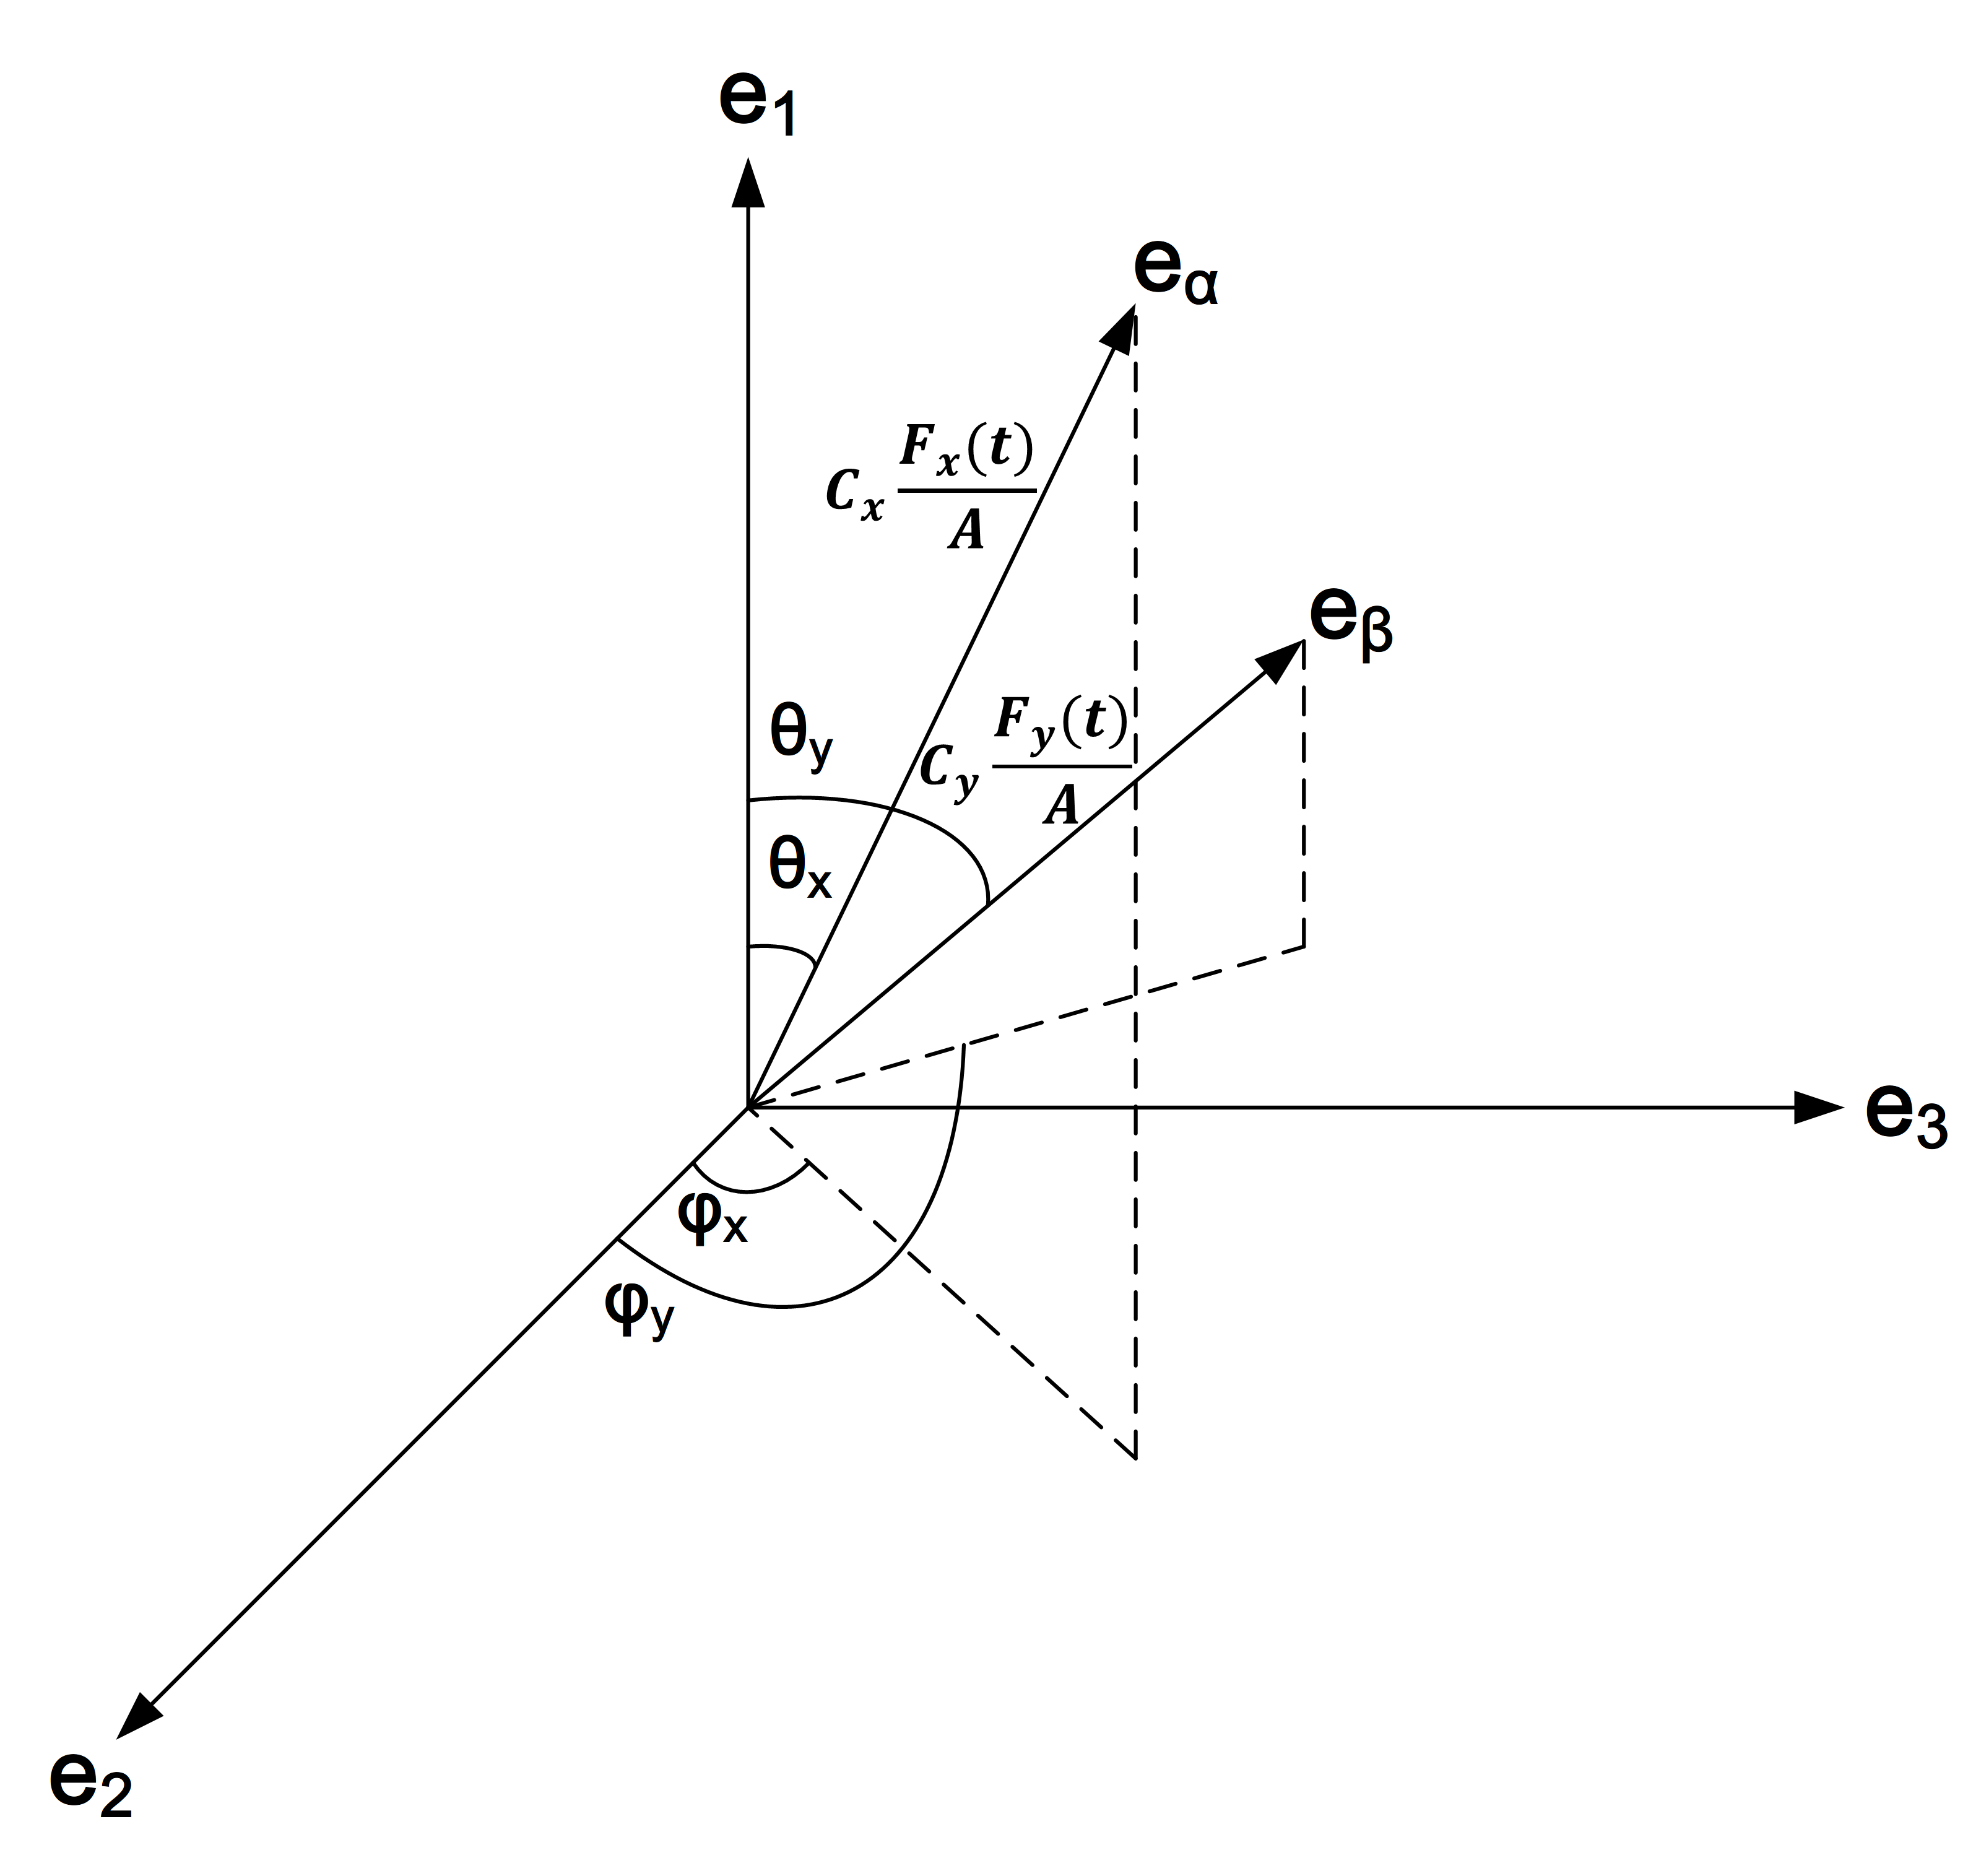
\includegraphics[width=0.7\textwidth]{figures//xab.png} 
  	\caption{Loading in 3 different directions}
  	\label{xab}
  \end{figure}
\end{frame}	

\begin{frame}
	\frametitle{Multi-dimensional application}
\begin{figure}[!h]
	\centering
	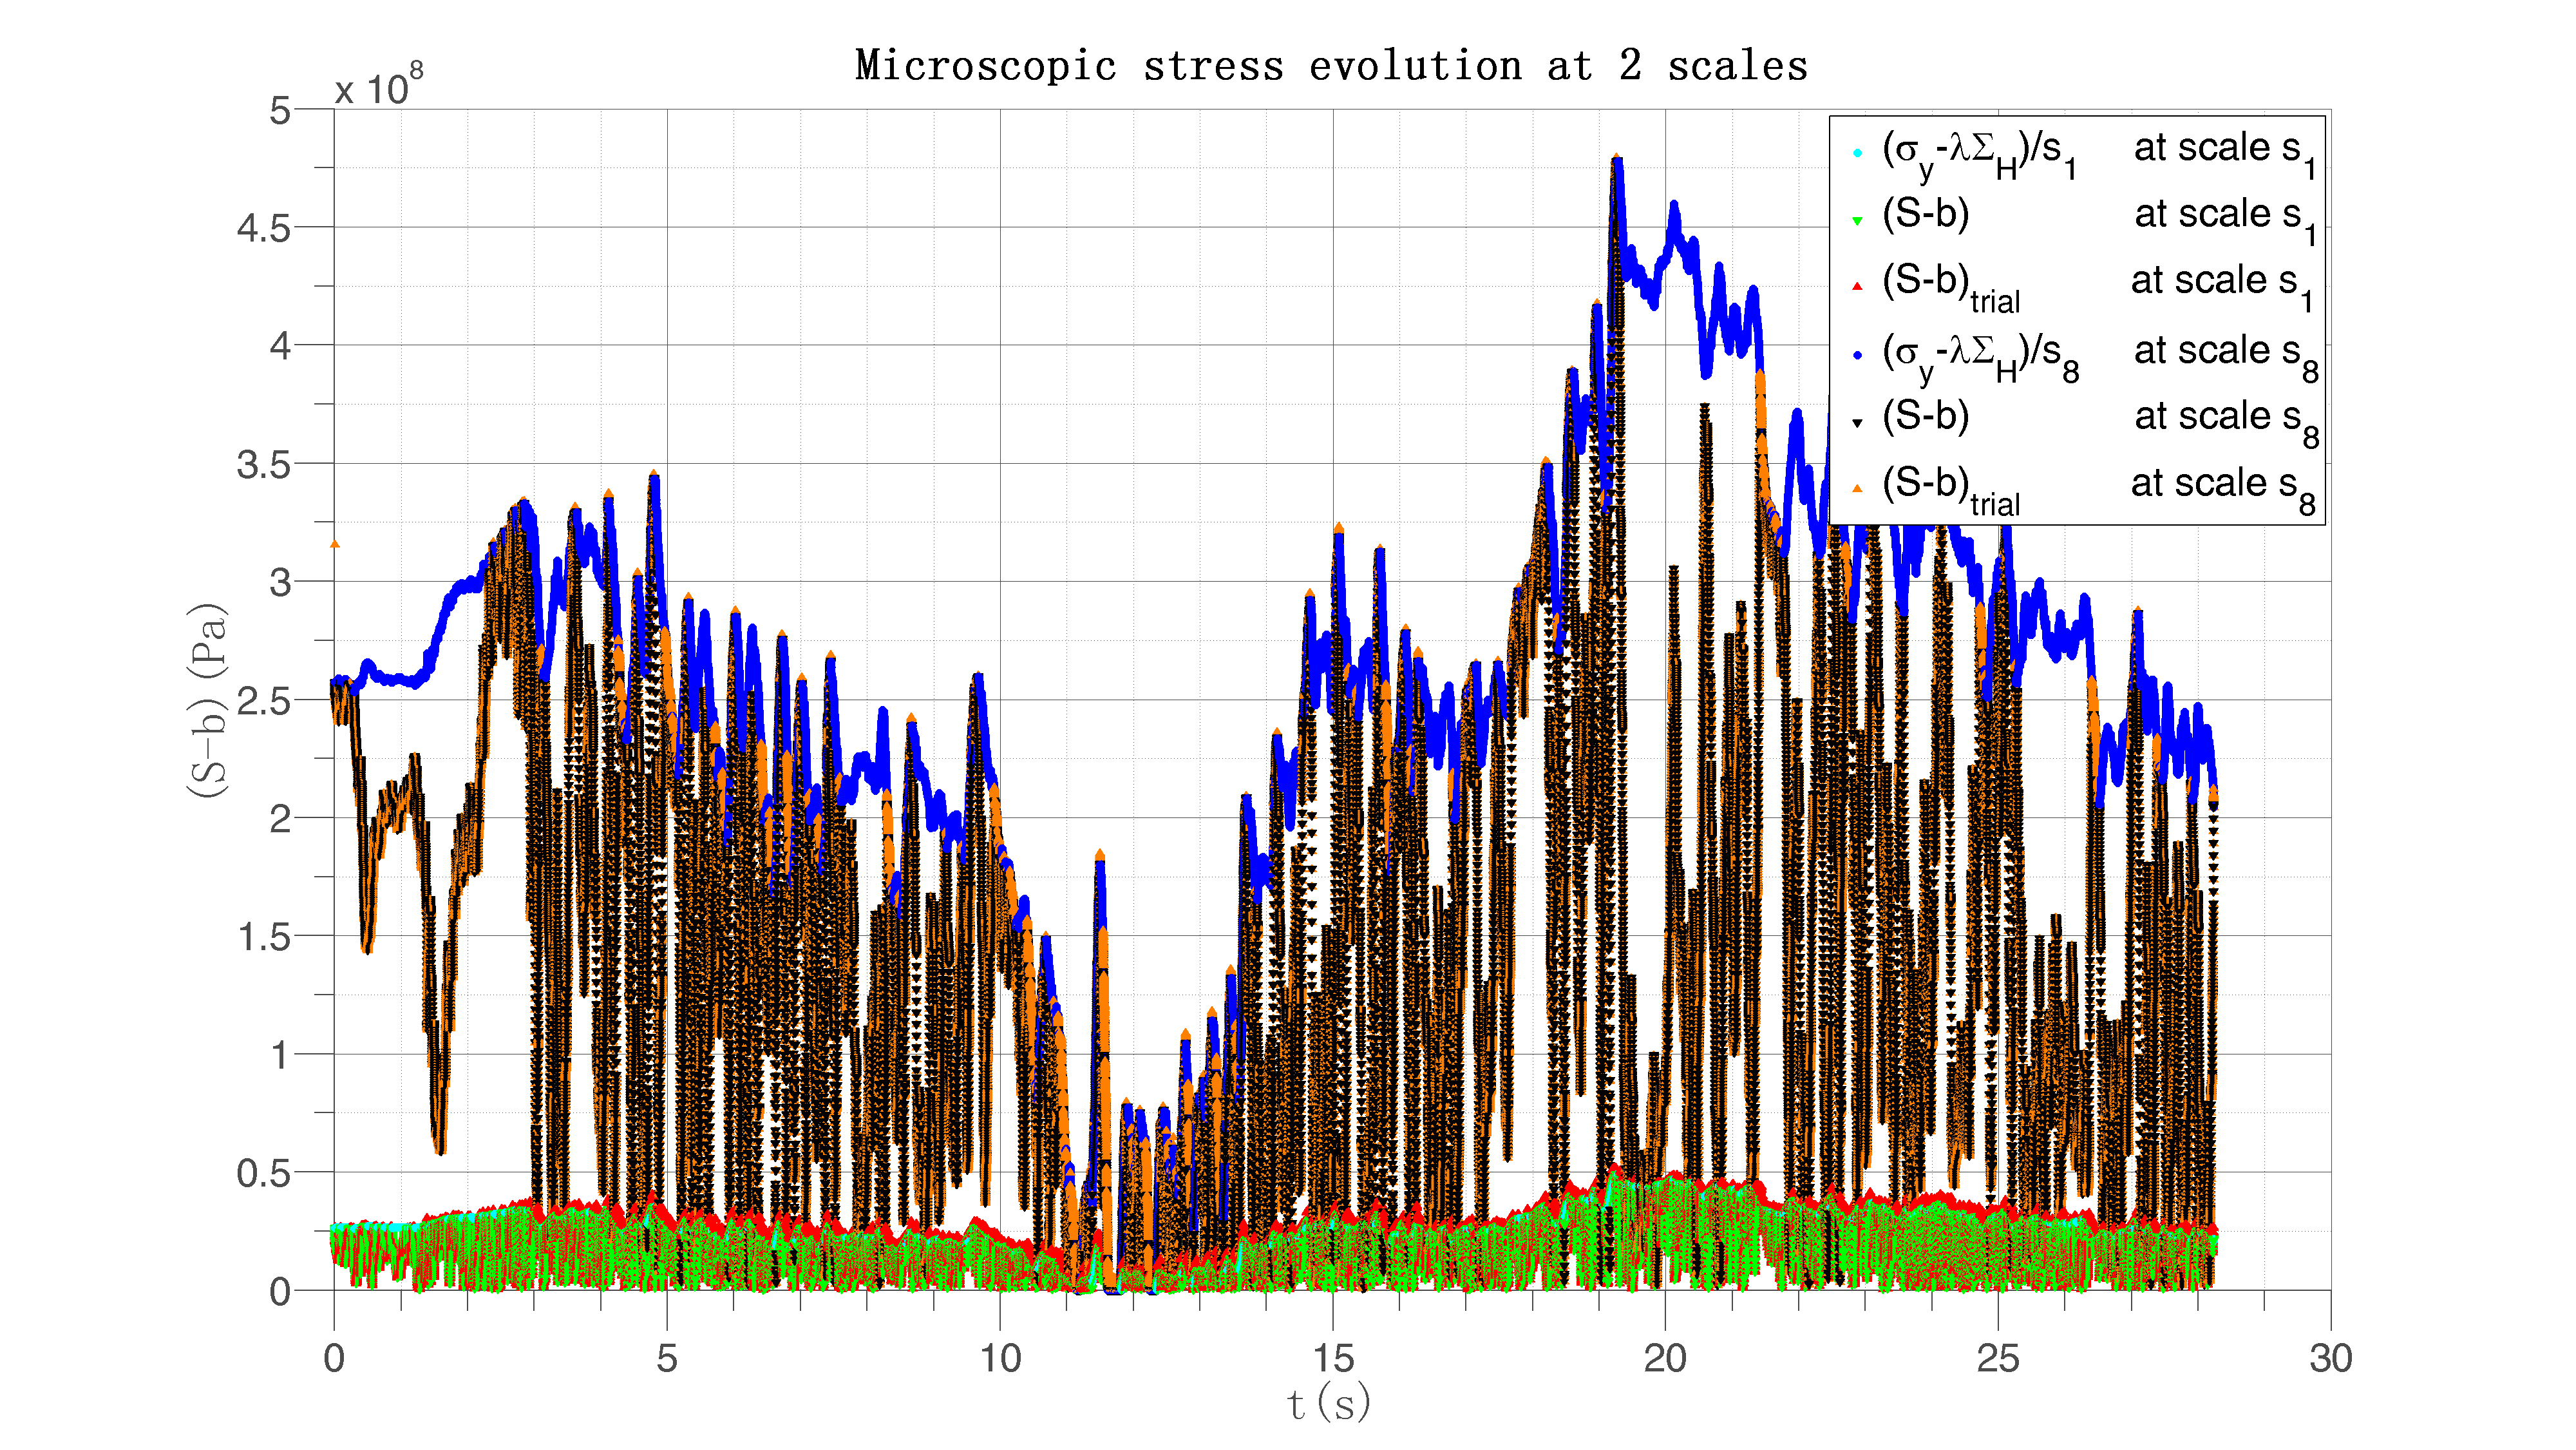
\includegraphics[width=\textwidth]{figures//trialreal3d.png} 
	\caption{$\left\| \uline{\uline{S}}-\uline{\uline{b}}\right\|_{trial}$ and $\left\| \uline{\uline{S}}-\uline{\uline{b}}\right\|$ evolution with time under different weakening scales in PSA load history}
	\label{trialreal3d2}
\end{figure} 
\end{frame}	
\begin{frame}
	\frametitle{Multi-dimensional application}
\begin{figure}[!h]
	\centering
	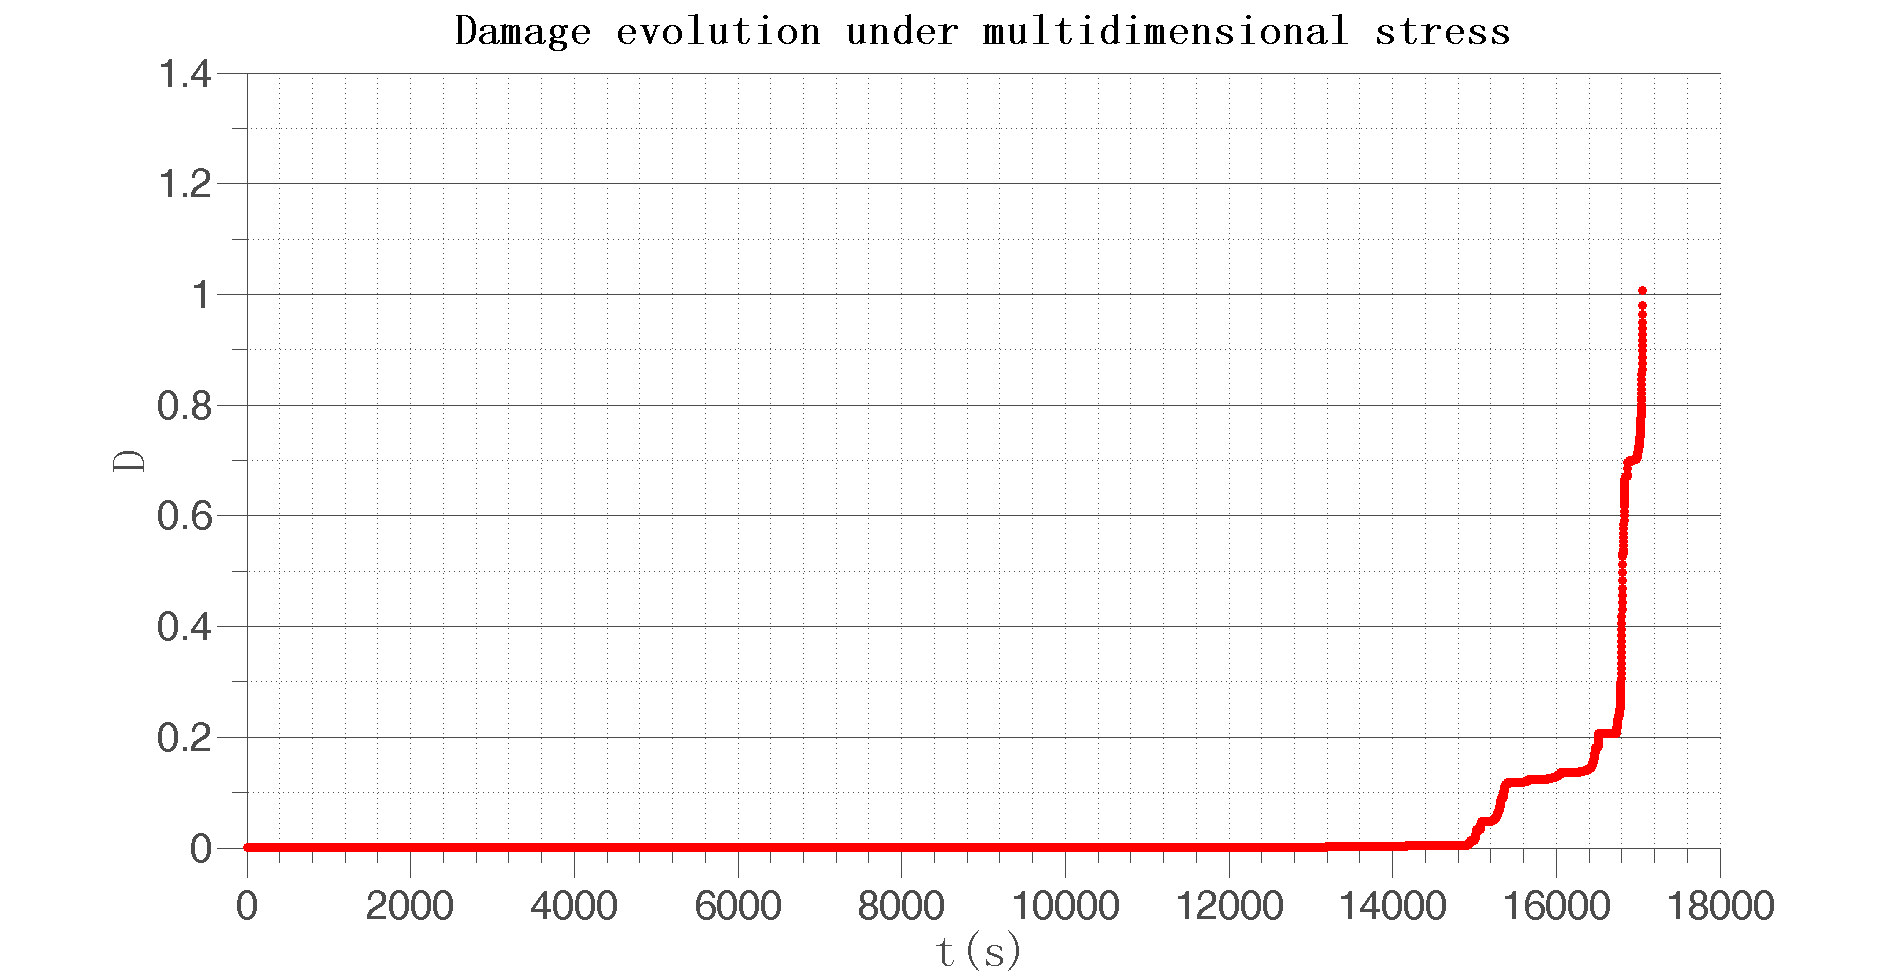
\includegraphics[width=\textwidth]{figures//damage3d2.png} 
	\caption{Damage evolution under multidimensional stress}
	\label{dam3d}
\end{figure}
\end{frame}	


\begin{frame}
	\frametitle{Discussion}	
		\begin{exampleblock}{Discussion}
\begin{enumerate}
	\item We work on the stress tensor directly in 3D analysis in stead of using the multidimensional equivalent stress.
	
	\vspace{6pt}
	\item   The energy based fatigue approach takes into account impurities and hardness in the material and is applicable to any type of micro plasticity law and multiaxial load geometry.
	
	\vspace{6pt}
	\item The small step-by-step strategy does not ignore small fluctuations in load history and the big stress effect is magnified which reflects the real situation.
	
\end{enumerate}
\end{exampleblock}
\end{frame}	


\begin{frame}
	\frametitle{}	
	\begin{exampleblock}{}
		{
			\Huge $$Thanks \, for \, your \, attention!$$
		}	  
	\end{exampleblock}
\end{frame}			
\end{document}

